\chapter{Analisi}
\label{capitoloanalisi}
Questo capitolo illustra i dati collezionati e i risultati otteniti tramite il processo di analisi proposto per studiare la migrazione altamente specializzata a partire da fonti di dati non convenzionali.  
La prima parte del capitolo descrive il dataset collezionato attraverso Academic Reasearch Access e propone lo studio dell'utenza Crunchbase. 
In seguito, il capitolo descrive i risultati delle analisi svolte sulle scorte (Sezione \ref{sec:analisi_scorte}) e sui flussi (Sezione \ref{sec:analisi_flussi}). In entrambe i casi, viene prima analizzato l'insieme di dati collezionato per determinare le zone più rappresentate.
Per le scorte vengono analizzati alcuni casi di studio specifici, le scorte in Italia e gli emigrati italiani, le scorte in Gran Bretagna e gli emigrati britannici ed infine le scorte di nazionalità Europea in nord America e le scorte di nazionalità nord americana in Europa.
I flussi vengono analizzati nella loro totalità e su diversi piani di aggregazione per zone geografiche, con due casi di studio dedicati all'Italia e alla Gran Bretagna. 

Per ogni analisi affrontata è stato calcolato:
\begin{itemize}
    \item Pearson: Correlazione di Pearson calcolata sugli insiemi forniti.
    \item Spearman: Indice di Spearman calcolato sugli insiemi forniti.
    \item PearsonLog: Correlazione di Pearson calcolata sugli insiemi forniti in scala logaritmica.
    \item PearsonLog(Risorsa): Correlazione di Pearson calcolata sugli insiemi forniti, e l'insieme ``Risorsa'' è in scala logaritmica.
\end{itemize}
Il campo ''Risorsa'' può avere quattro valori ovvero CB per Crunchbase, ESTAT per Eurostat, UN per United Nations e Official per l'unione di UN e Eurostat.


\section{Confronto tra metodi di collezione} 
\label{validazionedaticollezionati}

Le scorte dal 2010 al 2020 ottenute attraverso l'impiego del Custom Query Builder (CQB) - Sezione \ref{customquerybuilder} -  e i dati ufficiali ottenuti attraverso l'Academic Research Access (Sezione \ref{academic_access_section}) vengono confrontati nella Figura \ref{fig:scrapervsapi}. Le nazionalità per cui i dati sono stati confrontati sono Austria, Belgio, Francia, Germania, Grecia, Irlanda ed Italia. Vengono calcolate anche le correlazioni. Osserviamo sia dal grafico che dalle correlazioni che le scorte ottenute tramite il CQB sono molto diverse da quelle dell'accesso accademico, con valori molto minori tramite CQB. Quindi il resto delle analisi vengono eseguito sui dati da Academic Research Access. 

\begin{figure}[t]
    \centering
    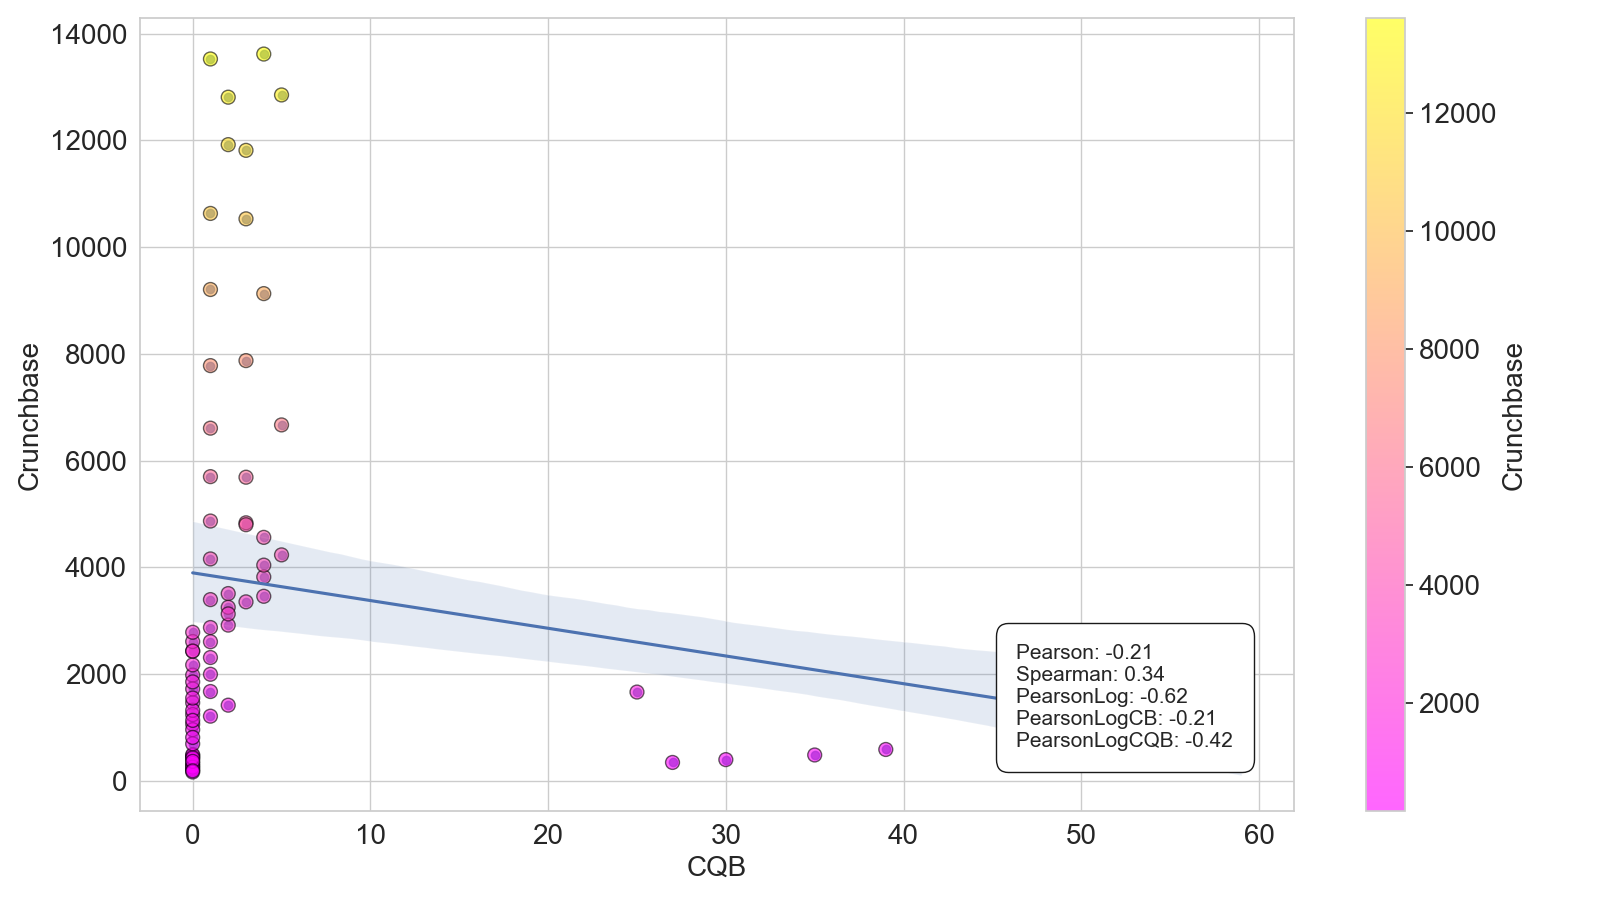
\includegraphics[width=1.0\textwidth]{images/crunchbase_academic_access/myplot.png}
    \caption{Confronto delle scorte ottenute dal Custom Query Builder e dall'Academic Reasearch Access per i paesi selezionati.}
    \label{fig:scrapervsapi}
\end{figure}


\section{Descrizione del dataset collezionato}
\label{sec:datasetcollezzionato}
L'intero dataset generato attraverso l'Academic Research Access contiene 1.288.646 profili utente.
Viene effettuata un'analisi per determinare gli stati per cui Crunchbase è più rappresentato. La prima fase di analisi viene effettuata attraverso una mappa di calore dell'utenza di Crunchbase per visualizzare quali sono le zone geografiche per cui la piattaforma è più utilizzata (Figure \ref{fig:crunchuserbaseheatmap}). La seconda fase prevede la creazione di un grafico che indica l'utenza nel tempo per i primi dieci stati per numero di utenti (Figura \ref{fig:lineplotutenza}). Entrambi i grafici sono stati realizzati usando i dati relativi a tutta l'utenza Crunchbase altamente qualificata per periodo compreso tra il 2010 ed il 2020. 
\begin{figure}[tb]
    \centering
    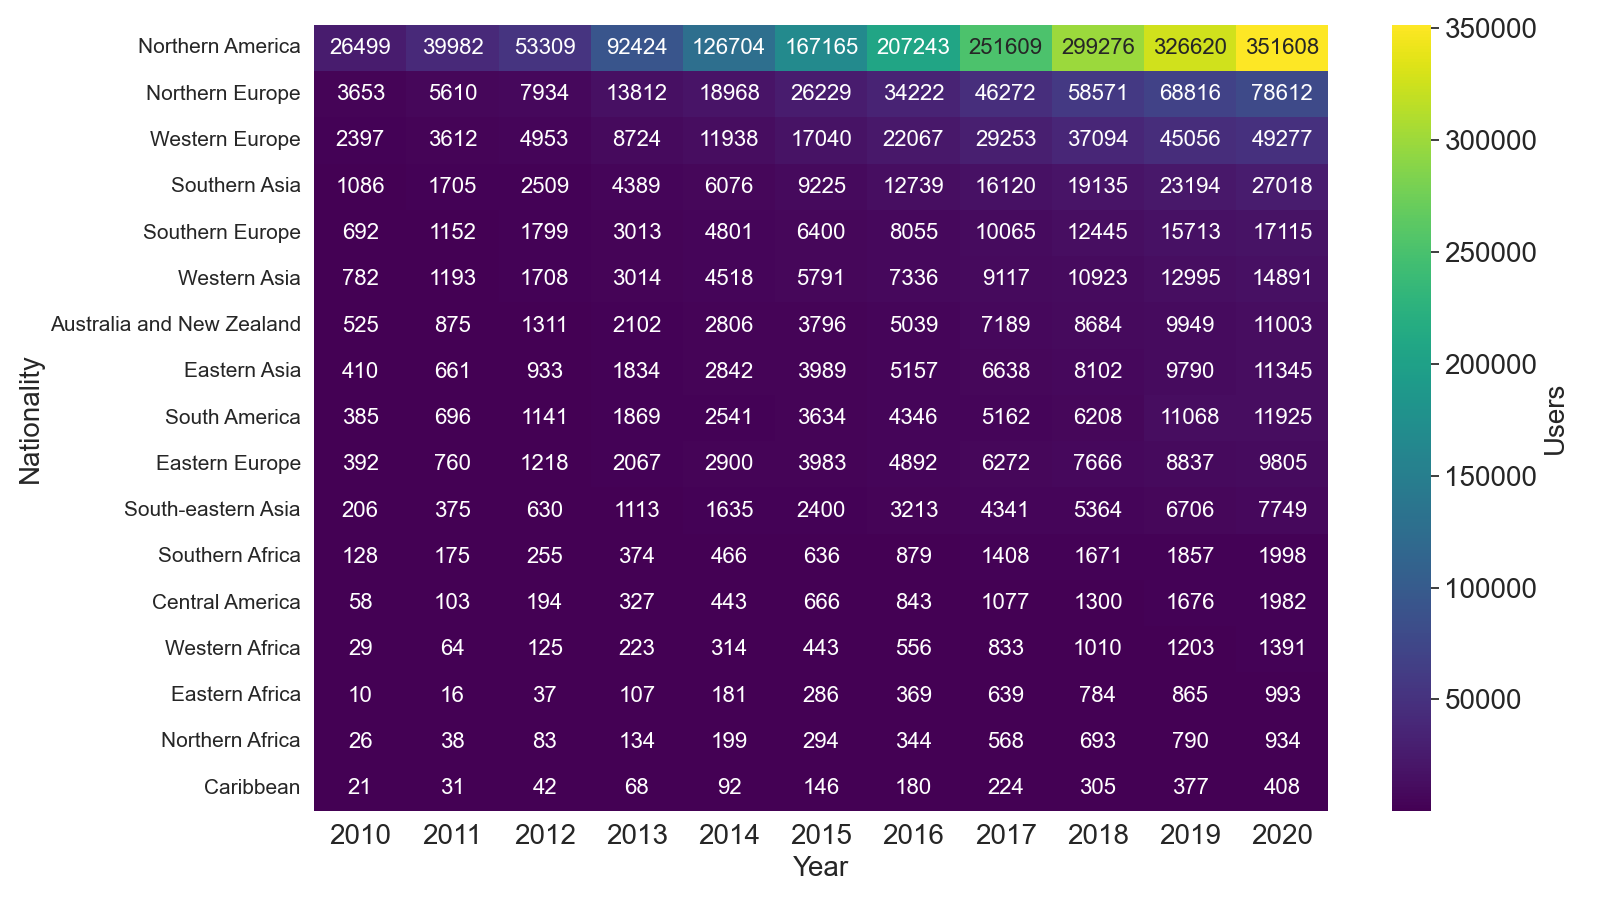
\includegraphics[width=\textwidth]{images/crunchbase_userbase/heatmap2.png}
    \caption{Utenza annuale di Crunchbase nel periodo 2010-2020 aggregata per zone geografiche}
    \label{fig:crunchuserbaseheatmap}
\end{figure}

La Figura \ref{fig:crunchuserbaseheatmap} mostra l'utenza annuale di Crunchbase (dal 2010 al 2020) in base alla nazionalità (inferita seguendo la definizione in Sezione \ref{preprocessing}). Si noti che le nazionalità sono state aggregate per sub continenti.
La crescita dell'utenza si osserva per tutti i paesi, in tutti i dieci anni osservati. Tuttavia, si nota che l'incremento nel numero di utenti è fortemente dipendente  dalle zone geografiche. L'America del nord è la zona con più utenti, seguita, seppur con larga differenza, dal nord e ovest Europa, e dal sud e ovest Asia. 

La Figura \ref{fig:lineplotutenza} mostra l'utenza Crunchbase dei dieci stati con più utenti sulla base della nazionalità. 
Per tutti e dieci i paesi si osserva una linea di valori monotona crescente, che indica che nel tempo la piattaforma è sempre più usata. 
\begin{figure}[tb]
\hfill
    \centering
    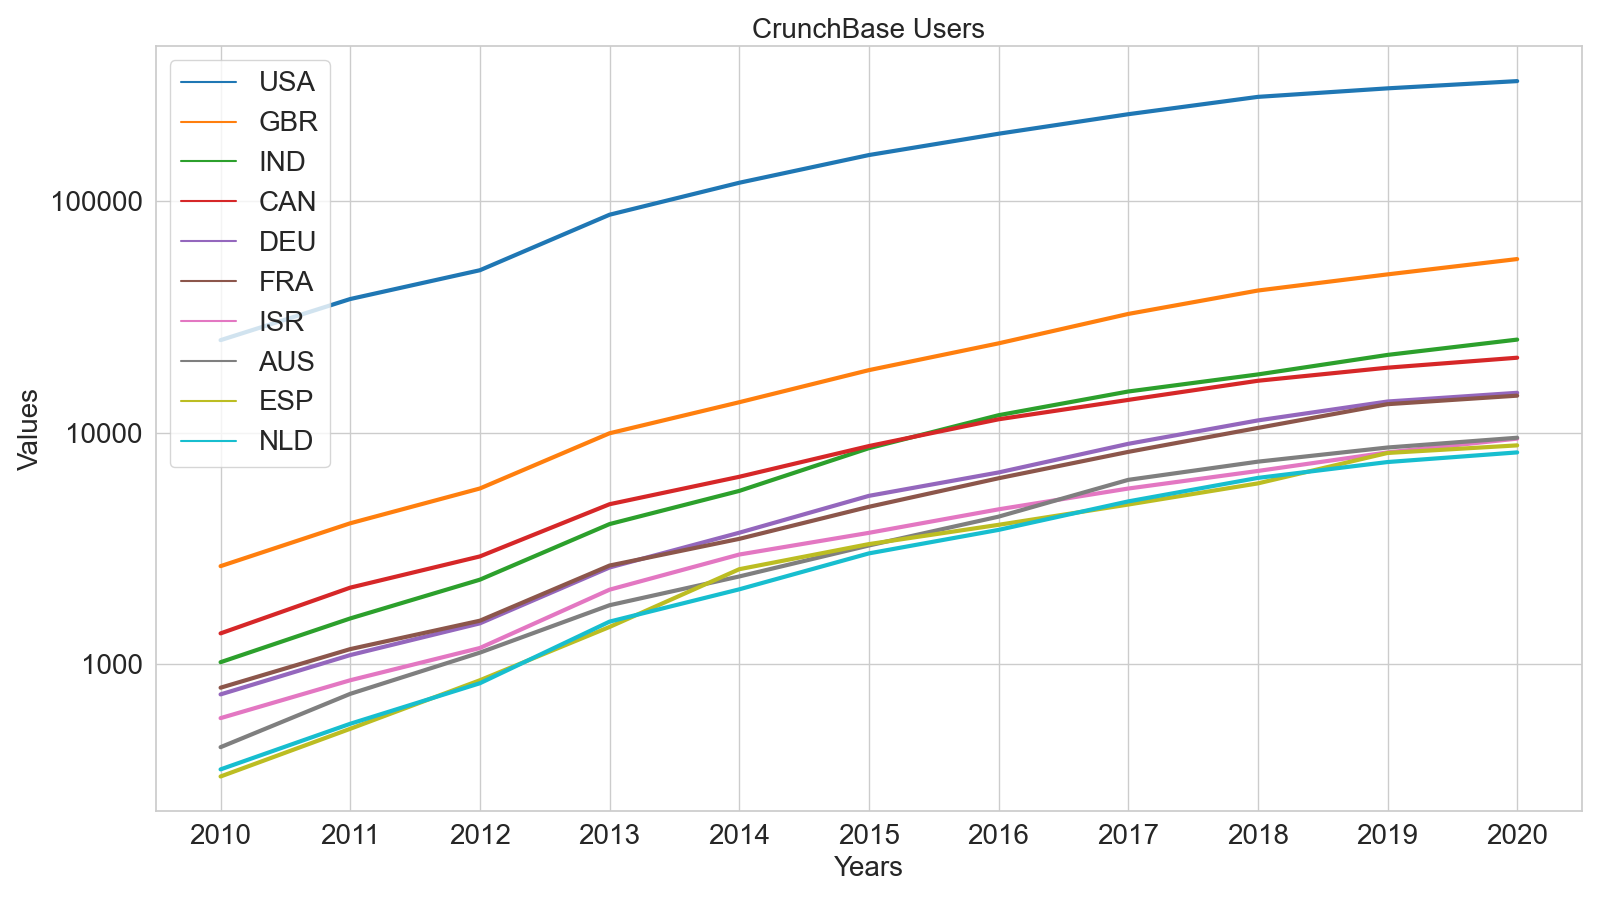
\includegraphics[width=1.0\textwidth]{images/crunchbase_userbase/lineplotlog.png}
    \caption{Trend utenza annuale di Crunchbase dal 2010 al 2020 per primi dieci paesi per numero di utenti totali al 2020.}
    \label{fig:lineplotutenza}
\end{figure}


I dati relativi a scorte e flussi estratti durante la fase di preprocessing (Sezione \ref{preprocessing}) sono stati analizzati per comprenderne la cardinalità. Il numero di scorte collezionate attraverso l'accesso accademico a Crunchbase è di 26.432. Ogni scorta è rappresentata da una tripla \texttt{nazionalità-statoScorte-anno}. 


I flussi, invece, hanno una cardinalità di 6716 combinazioni rappresentate da una tripla \texttt{origine-destinazione-anno}. Inoltre, ogni combinazione ha un valore per i residenti ed uno per i cittadini. 

\section{Analisi delle scorte}
\label{sec:analisi_scorte}
In questa sezione vengono analizzate le scorte di migranti di Crunchbase. 
Durante la fase iniziale, abbiamo analizzato le scorte lungo tutto l'arco temporale coperto dai dati (dal 2010 al 2020). 
Le scorte di Crunchbase sono state confrontate, mediante il calcolo della correlazione di Pearson e di Spearman, con le scorte in UN per gli anni 2010, 2015 e 2020. 
Per la visualizzazione dei risultati sono stati realizzati grafici di dispersione.

Per approfondire l'analisi, sono stati realizzati tre casi di studio. I primi due studi riguardano gli emigrati e immigrati italiani e britannici rispettivamente. Infine, il terzo caso analizzato si concentra sugli stati europei e nord americani. 

\subsection{Dati di Crunchbase}
\label{stockCrunchbase}
\begin{figure}[t]
    \centering
    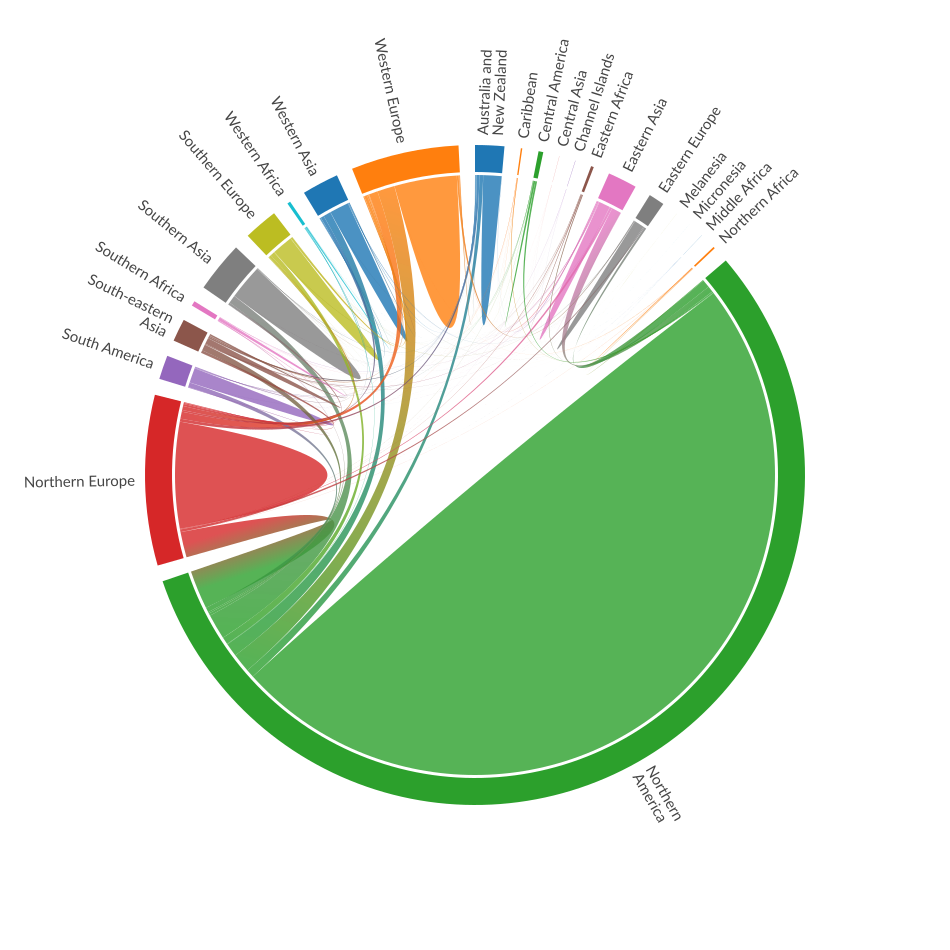
\includegraphics[width=\textwidth]{images/SVG/Chords/stocks/stock_chord_all.png}
    \caption{Scorte di migranti ottenute da Crunchbase sommate per il periodo 2010-2020.}
    \label{fig:chordCrunchbase_stock_all}
\end{figure}

Le scorte migratorie in Figura \ref{fig:chordCrunchbase_stock_all} sono in accordo con l'analisi dell'utenza Crunchbase effettuata in Sezione \ref{sec:datasetcollezzionato}. Ogni sezione del perimetro rappresenta una zona geografica, ogni arco rappresenta un numero di scorte di quella nazionalità rilevate nell'altro paese. Gli archi hanno dimensione differente in base alla dimensione delle scorte rilevate. La maggior parte degli utenti è rappresentato da nativi nord-americani residenti in nord America (non migranti). Osservando le singole zone, gli emigrati nord americani risiedono nell'ovest e nel nord Europa, e nel sud e est Asia. Inoltre, il nord America sembra accogliere il maggior numero di immigrati provenienti da tutte le zone, seppur in diversa misura.
Gli utenti del nord Europa e Europa dell'ovest sono rispettivamente il secondo e terzo gruppo più rappresentato. In entrambi i casi, così come per le altre zone, la maggior parte degli utenti è rappresentata da nativi. Nonostante ciò, parte degli utenti del nord Europa sembra essere emigrata in ovest Europa, e viceversa. 

\begin{figure}[htbp]
    \centering
    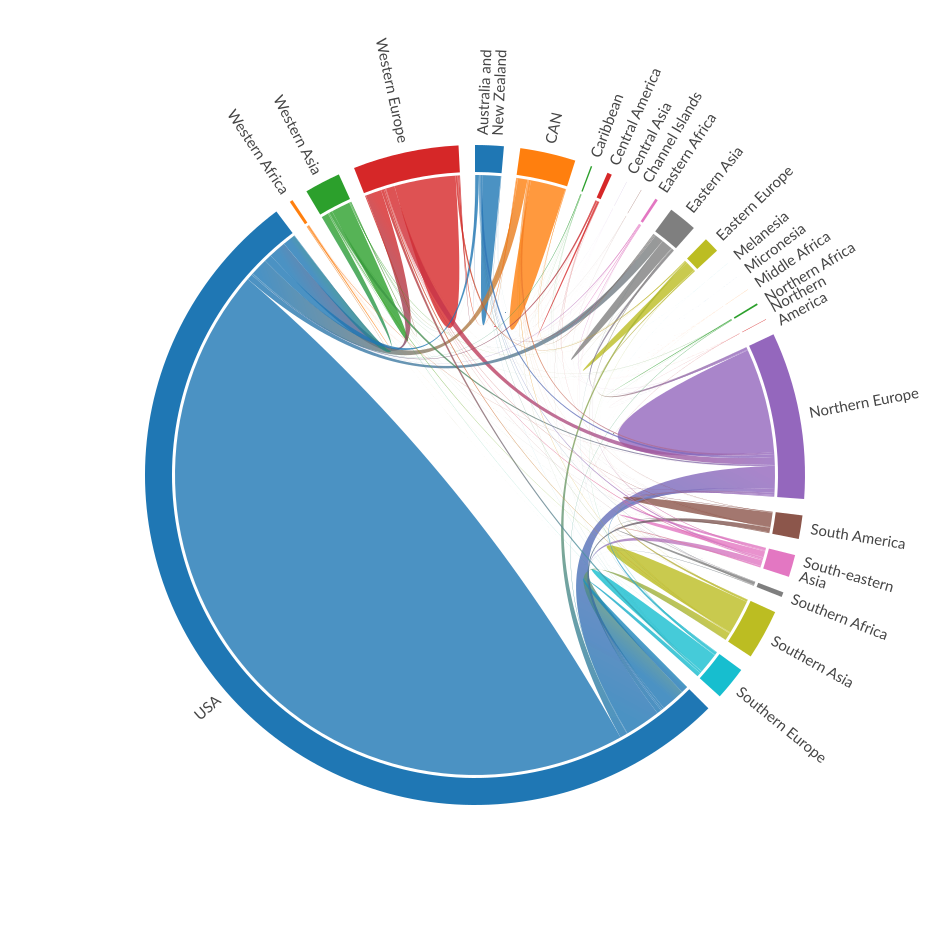
\includegraphics[width=0.9\textwidth]{images/SVG/Chords/stocks/stock_chord_USA_CAN_separate.png}
    \caption{Scorte migratorie aggregate per zone più Stati Uniti d'America e Canada. Le scorte sono sommate per il periodo dal 2010 al 2020.}
    \label{fig:chordCrunchbase_stock_usa_can}
\end{figure}

\begin{figure}[htbp]
    \centering
    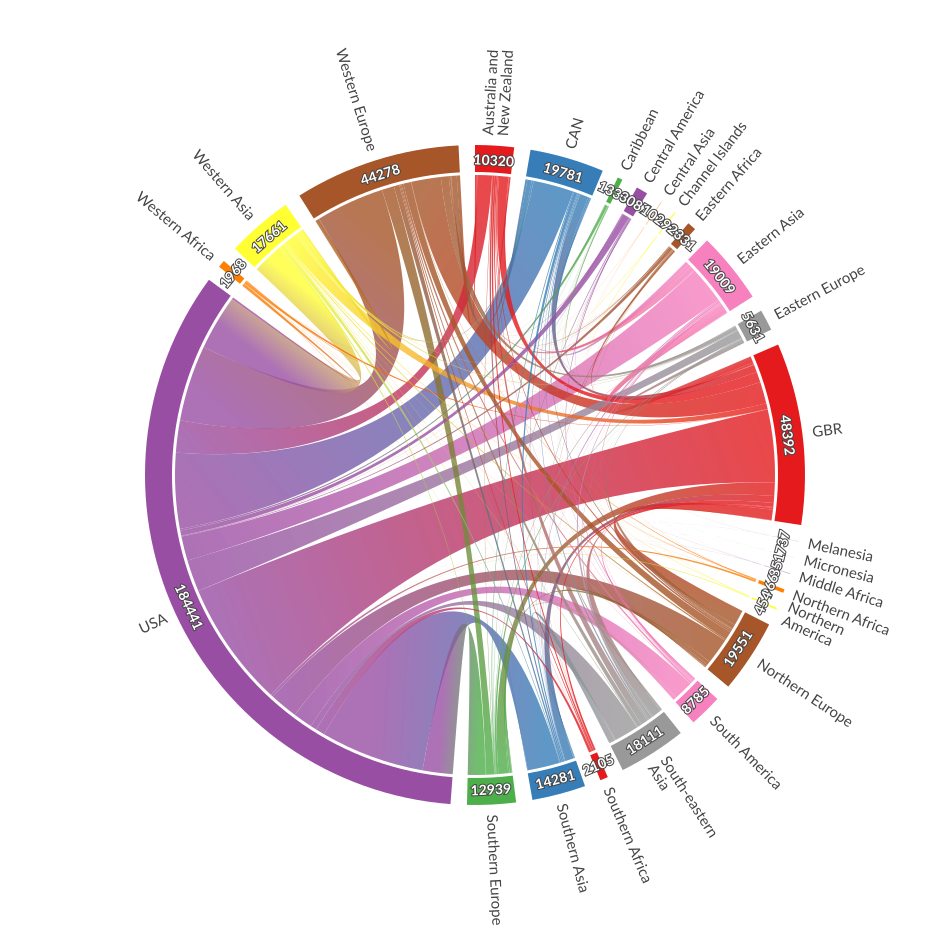
\includegraphics[width=0.9\textwidth]{images/SVG/Chords/stocks/stock_chord_USA_CAN_GBR_separate.png}
    \caption{Crunchbase scorte con Stati Uniti, Canada and Gran Bretagna separati dall'aggregazione.}
    \label{fig:chordCrunchbase_stock_usa_can_gbr}
\end{figure}

La Figura \ref{fig:chordCrunchbase_stock_usa_can} rappresenta le scorte migratorie, sommate dal 2010 al 2020, considerando Stati Uniti d'America e Canada come zone a sé stanti. Ogni sezione del perimetro del grafico rappresenta uno degli stati (USA o CAN) o la zona geografica.
Sebbene il grafico sia molto simile a quello in Figura \ref{fig:chordCrunchbase_stock_all}, sottolinea la differenza nel numero di immigrati/emigrati tra Stati Uniti d'America e Canada e tutte le altre zone. 


La Figura \ref{fig:chordCrunchbase_stock_usa_can_gbr} rappresenta tutte le scorte migratorie internazionali considerando Stati Uniti d'America, Canada e Gran Bretagna come zone a sé stanti, sommate dal 2010 al 2020. Gli archi hanno dimensione differente in base alla dimensione delle scorte rilevate su Crunchbase.  A differenza delle Figure \ref{fig:chordCrunchbase_stock_usa_can} e \ref{fig:chordCrunchbase_stock_all} i dati relativi a persone non migranti (e.g. Stati Uniti a Stati Uniti) non vengono considerati in questo grafico. Dalla figura si può notare la forte presenza di statunitensi in tutte le altre zone. Lo scambio di migranti più evidente è presente tra Stati Uniti e Gran Bretagna, a seguire ci sono in ordine il sud Asia, l'ovest dell'Europa e il Canada. L'Asia in tutte le sue coordinate presenta valori valori di scorte comparabili a quelli del nord Europa e del Canada.
\FloatBarrier
\subsection{Confronto Crunchbase con UN}

\label{UN_stock}
\begin{figure}[!h]
    \centering
    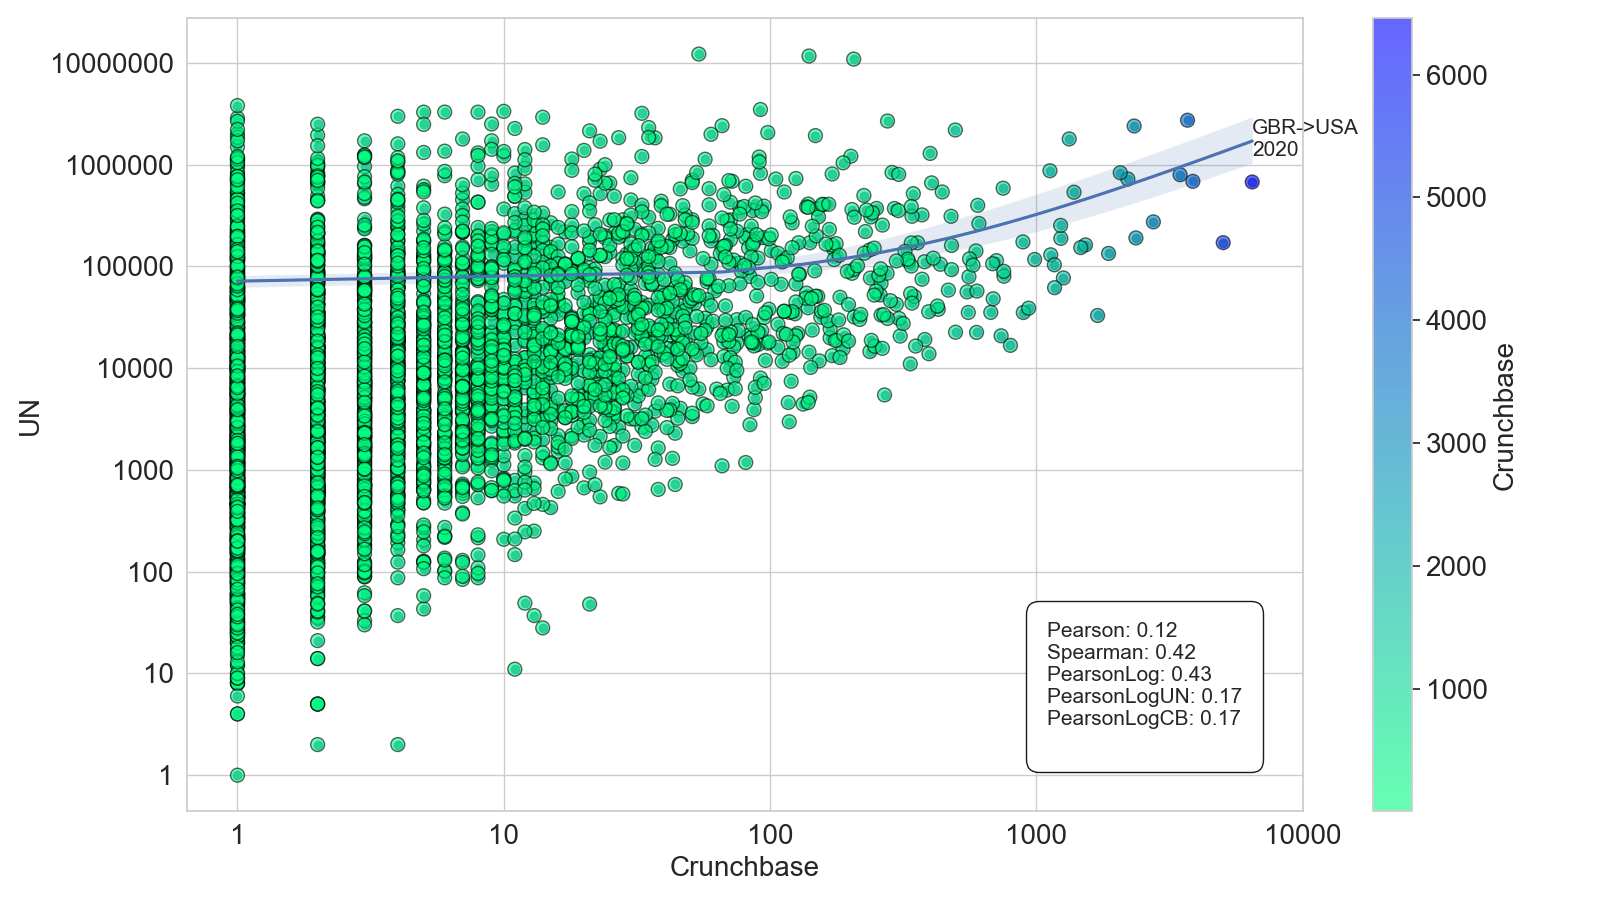
\includegraphics[width=0.8\textwidth]{images/Migration_Stocks/Migration Stocks.png}
    \caption{Confronto tra scorte di migranti in Crunchbase e UN. I dati sono per gli anni 2010, 2015 e 2020.}
    \label{fig:LogaritmicMigrationStocksScatterPlot}
\end{figure}
Il confronto delle scorte di Crunchbase con quelle di UN comporta la selezione delle combinazioni comuni di paesi. Inoltre, come descritto in precedenza (Sezione \ref{DatiTradizionali}), UN dispone di dati solo di dati quinquennali, nel nostro caso abbiamo selezionato gli anni 2010, 2015 e 2020. Questo duplice processo di selezione (coppie comuni e anni) riduce le combinazioni a 5295 (-21137).
Il grafico in Figura  \ref{fig:LogaritmicMigrationStocksScatterPlot} mostra la correlazione tra le scorte di Crunchbase e di UN, utilizzando una scala logaritmica per entrambi gli assi. Sull'asse x si hanno i dati Crunchbase, sull'asse y i dati UN. Il valore massimo ottenuto per le scorte Crunchbase è rappresentato accanto al punto relativo al suo valore, con la forma \textit{Nazionalità->Paese delle scorte Anno}. Nel riguardo in basso a destra sono presenti le varie correlazioni calcolate. La correlazione di Pearson è di 0.12, mentre l'indice di Spearman è di 0.42. Il coefficiente di Spearman ci indica che sia presente una correlazione debole tra le scorte in Crunchbase ed UN. Se si trasformano i dati delle scorte (UN e Crunchbase) in scala logaritmica per il calcolo della correlazione di Pearson, il valore è di 0.43 confermando il risultato ottenuto con il coefficiente di Spearman.
\FloatBarrier
\subsection{Caso di studio: Italia}
\label{itastock}
\begin{figure}[tbp]
  \centering
  \begin{minipage}[t]{0.8\textwidth}
    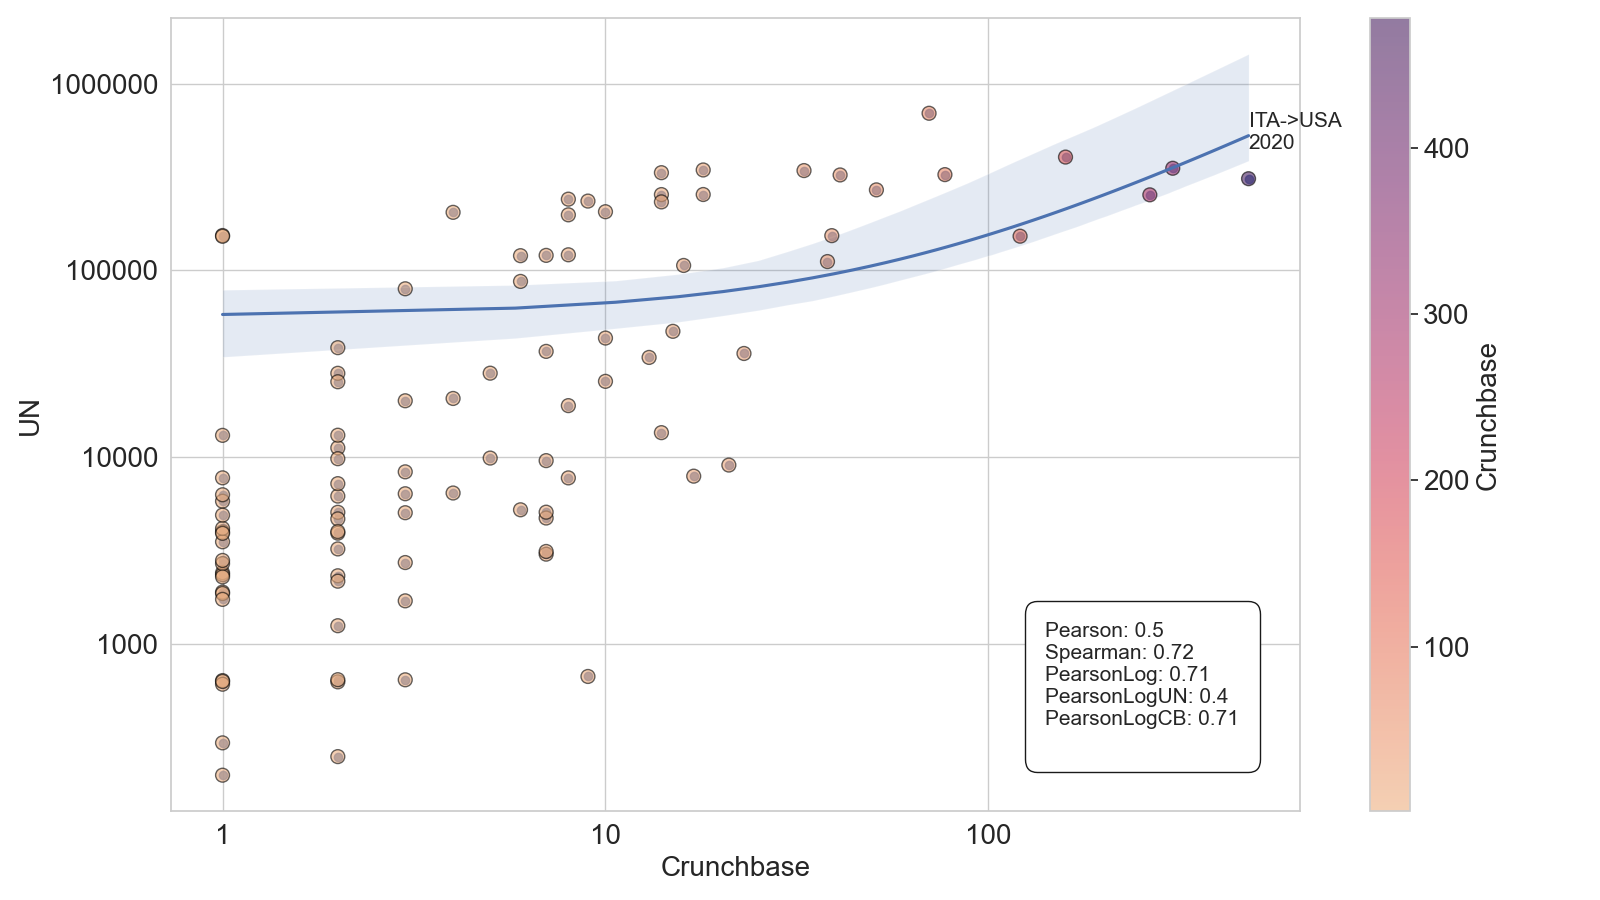
\includegraphics[width=\textwidth]{images/Migration_Stocks/ITA/Migration Stocks from ITA.png}
    \caption{Emigrati italiani nel mondo, confronto per gli anni 2010, 2015 e 2020 tra Crunchbase e UN.}
    \label{fig:MigrationstockswithItalianNationality}
  \end{minipage}
  %\hfill
  \begin{minipage}[b]{0.8\textwidth}
    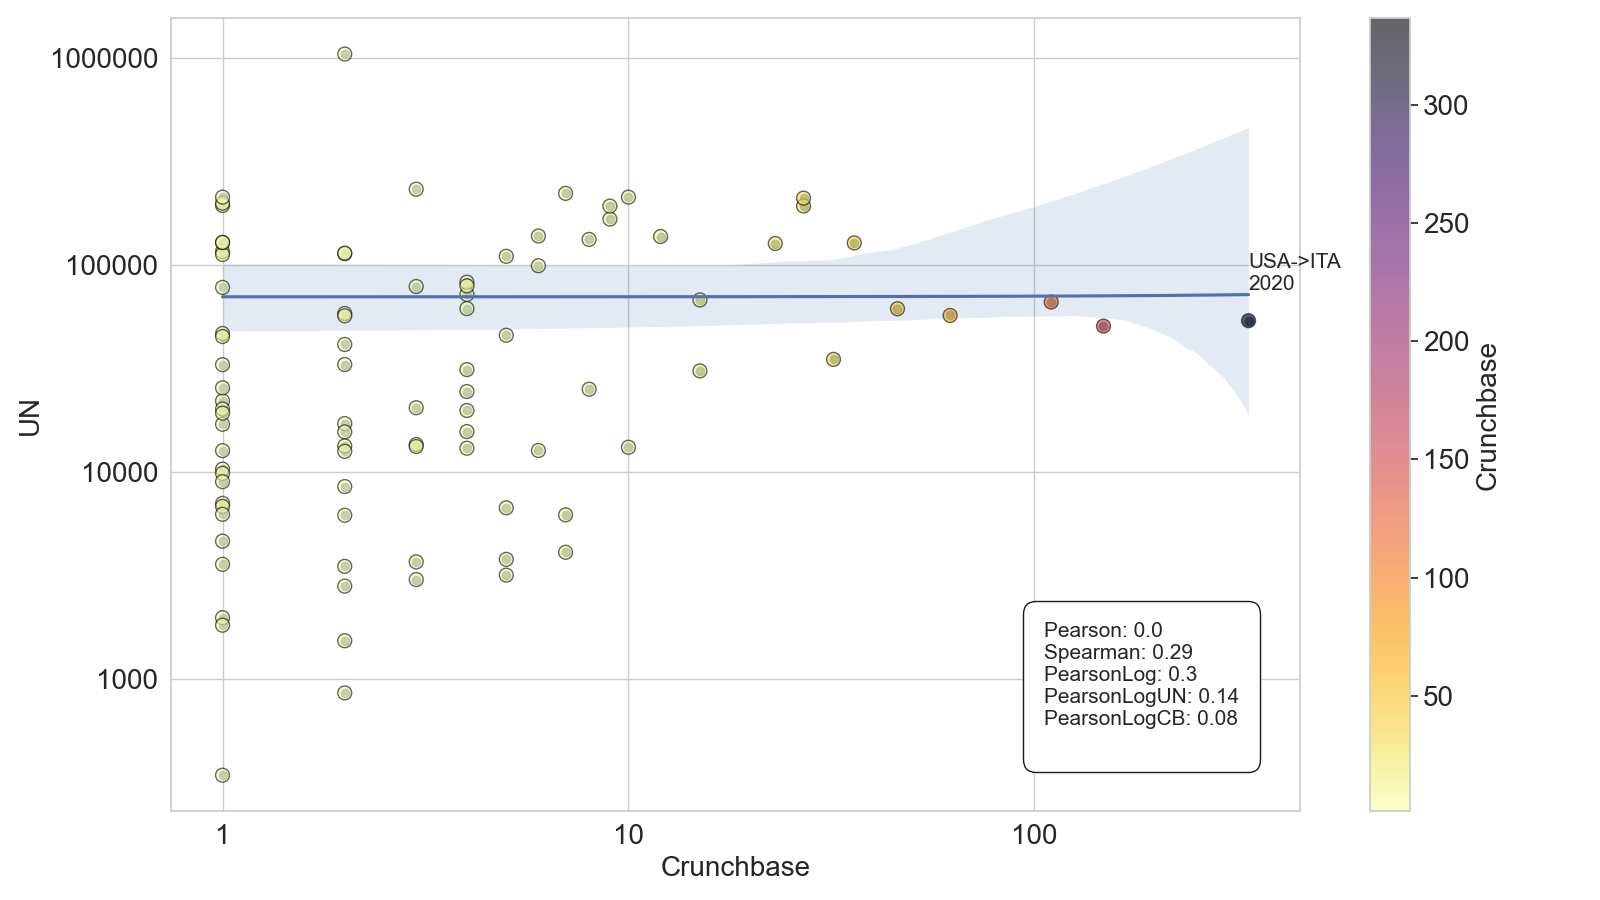
\includegraphics[width=\textwidth]{images/Migration_Stocks/ITA/Migration Stocks to ITA.png}
    \caption{Immigrati in Italia, confronto per gli anni 2010, 2015 e 2020 tra Crunchbase e UN. }
    \label{fig:MigrationstocktoItaly}
  \end{minipage}
\end{figure}

In questo studio vengono analizzate le scorte di migranti di nazionalità italiana nel mondo e le scorte di migranti in Italia. Lo studio è svolto per gli anni 2010, 2015 e 2020. 
La Figura \ref{fig:MigrationstockswithItalianNationality} mostra il confronto delle scorte di emigranti di nazionalità italiana tra UN e Crunchbase per gli anni 2010, 2015 e 2020. A destra la barra che indica i valori relativi ai vari colori, e il riquadro contenente le correlazioni calcolate. In basso il riquadro contenente le varie correlazioni calcolate. Come per il confronto precedente (Sezione \ref{UN_stock}), il valore massimo ottenuto per le scorte Crunchbase è rappresentato accanto al punto relativo al suo valore, con la forma \textit{Nazionalità->Paese delle scorte Anno}. La maggior parte delle scorte di italiani altamente qualificati per Crunchbase risiede negli Stati Uniti.
La correlazione di Pearson è 0,5 e l'indice di Spearman 0.72. La correlazione di Pearson, si eguaglia all'indice di Spearman (0.71) se le scorte in ingresso (UN e Crunchbase) sono poste in scala logaritmica. Questo ci indica una forte correlazione tra i dati UN e Crunchbase per le scorte di italiani fuori sede. 
Inoltre, il grafico in Figura \ref{fig:MigrationstocktoItaly} mostra il confronto tra le scorte di immigrati in Italia da Crunchbase e UN. La correlazione di Pearson in questo confronto ha valore zero, cioè indica che non c'è correlazione.
La correlazione di Pearson vede un incremento positivo fino a 0.3, se poniamo le scorte delle fonti (UN e Crunchbase) in scala logaritmica. L'indice di Spearman invece ha un valore di 0.29. Sebbene i valori dei coefficienti incrementino, non è sufficiente per determinare una correlazione debole.


\FloatBarrier
\subsection{Caso di studio: Gran Bretagna}
\label{gbrstock}
\begin{figure}[tbp]
  \centering
  \begin{minipage}[t]{1\textwidth}
    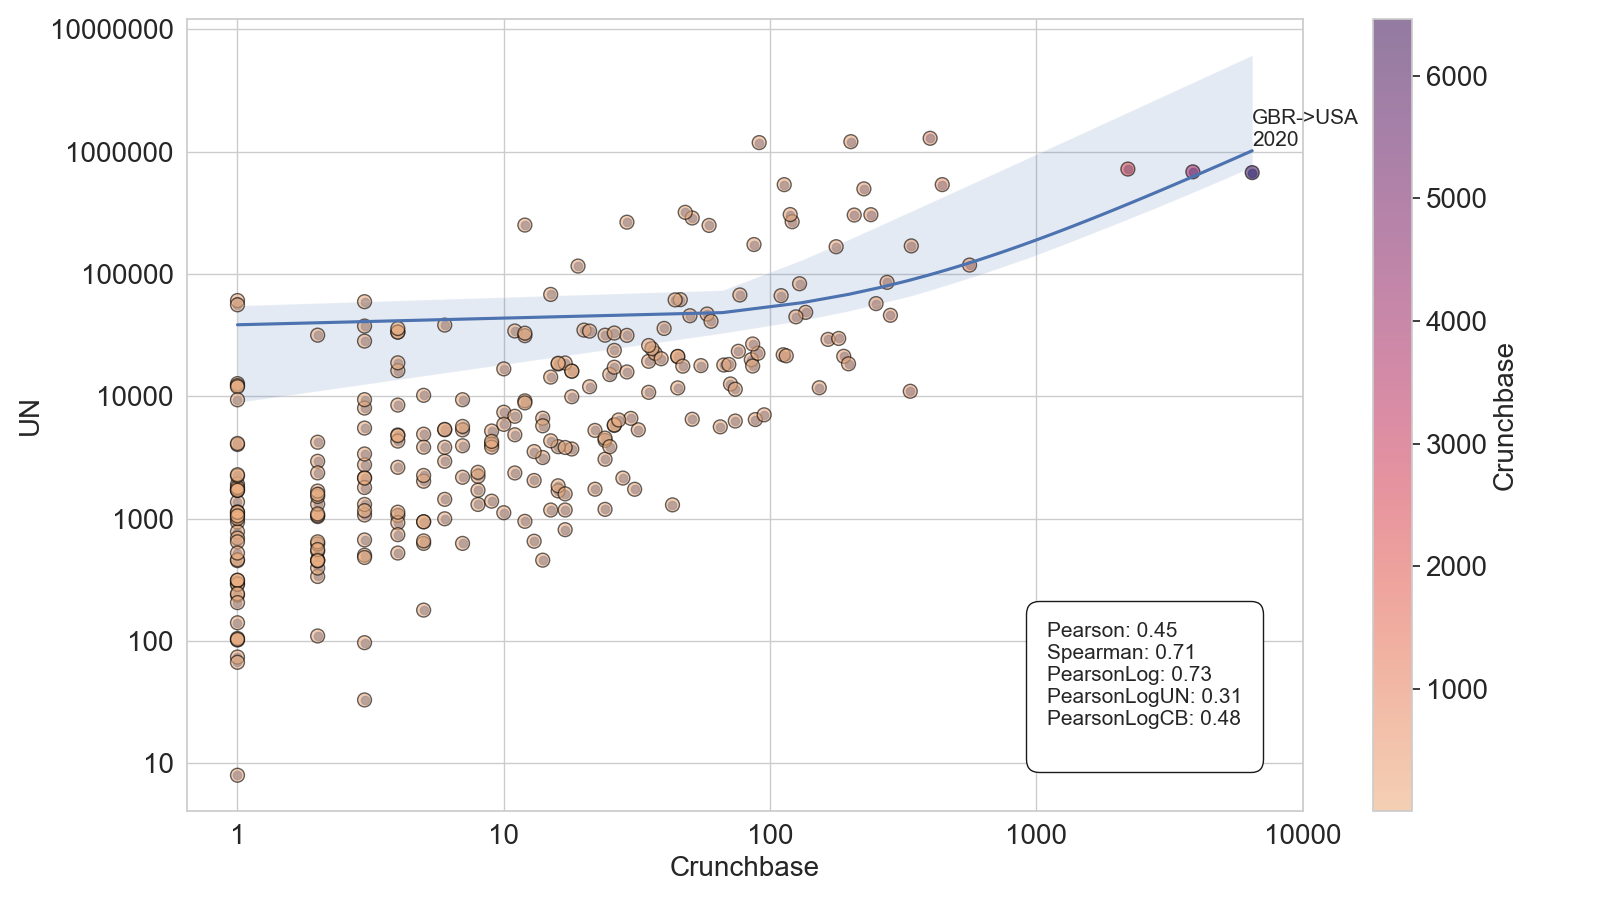
\includegraphics[width=\textwidth]{images/Migration_Stocks/GBR/Migration Stocks from GBR.png}
    \caption{Emigrati britannici nel mondo, confronto per gli anni 2010, 2015 e 2020 tra Crunchbase e UN.}
    \label{fig:Migrationstockfromgbr}
  \end{minipage}
  %\hfill
  \begin{minipage}[b]{1\textwidth}
    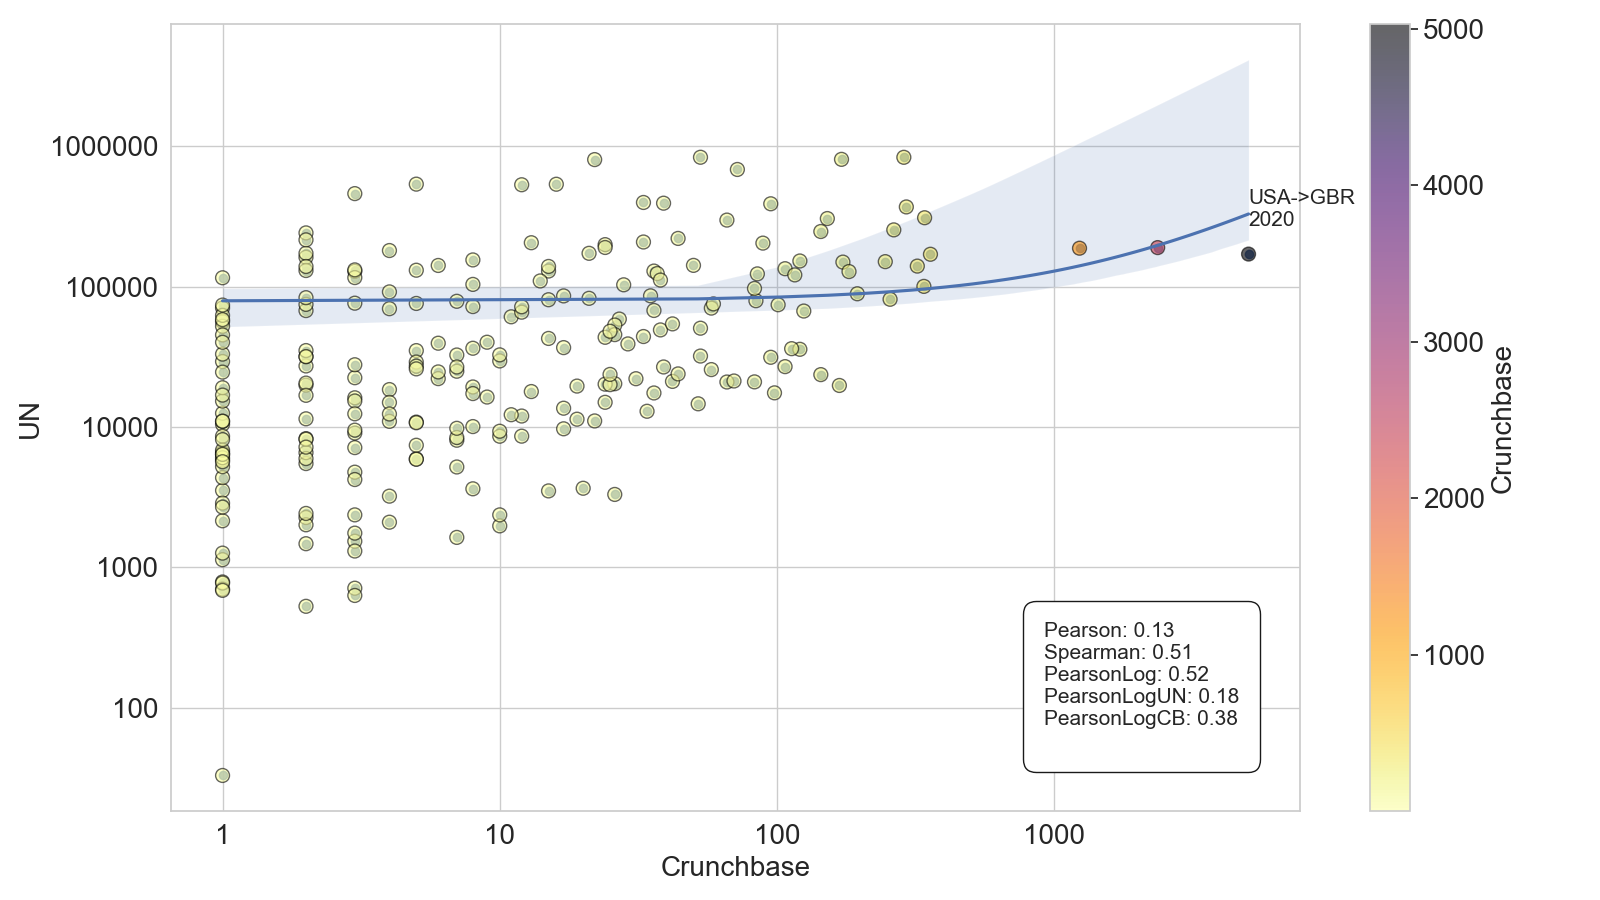
\includegraphics[width=\textwidth]{images/Migration_Stocks/GBR/Migration Stocks to GBR.png}
    \caption{Immigrati in Gran Bretagna, confronto per gli anni 2010, 2015 e 2020 tra Crunchbase e UN.}
    \label{fig:Migrationstocktogbr}
  \end{minipage}
\end{figure}

Le scorte relative a cittadini di nazionalità britannica emigrati, in Figura \ref{fig:Migrationstockfromgbr}, mostrano il valore massimo per gli Stati Uniti(circa 6.000). 
Entrambi gli indici di Pearson e Spearman mostrano correlazioni positive, di 0.45 e 0.71, rispettivamente.
La correlazione di Pearson calcolata con entrambe le variabili in scala logaritmica restituisce valori intorno a 0.73, denotando un buon livello di correlazione.

Per quanto riguarda le scorte migratorie della Gran Bretagna, il grafico in Figura \ref{fig:Migrationstocktogbr} mostra una correlazione di Pearson di 0.13 e dei valori più alti rispetto a quelli osservati per l'Italia (Figura \ref{fig:MigrationstocktoItaly}). L'indice di Spearman ha un valore di 0.51, quasi identico a quello di Pearson (0.52) quando le scorte sono poste in scala logaritmica. Le scorte più numerose in Gran Bretagna nel 2020 erano di nazionalità statunitense. Il valore massimo delle scorte di migranti in Gran Bretagna (5000) è tra i più altri osservati.

\FloatBarrier
\subsection{Caso di studio: Europa e nord America}
\label{europenordamstock}
\begin{figure}[tbp]
  \centering
  \begin{minipage}[t]{1\textwidth}
    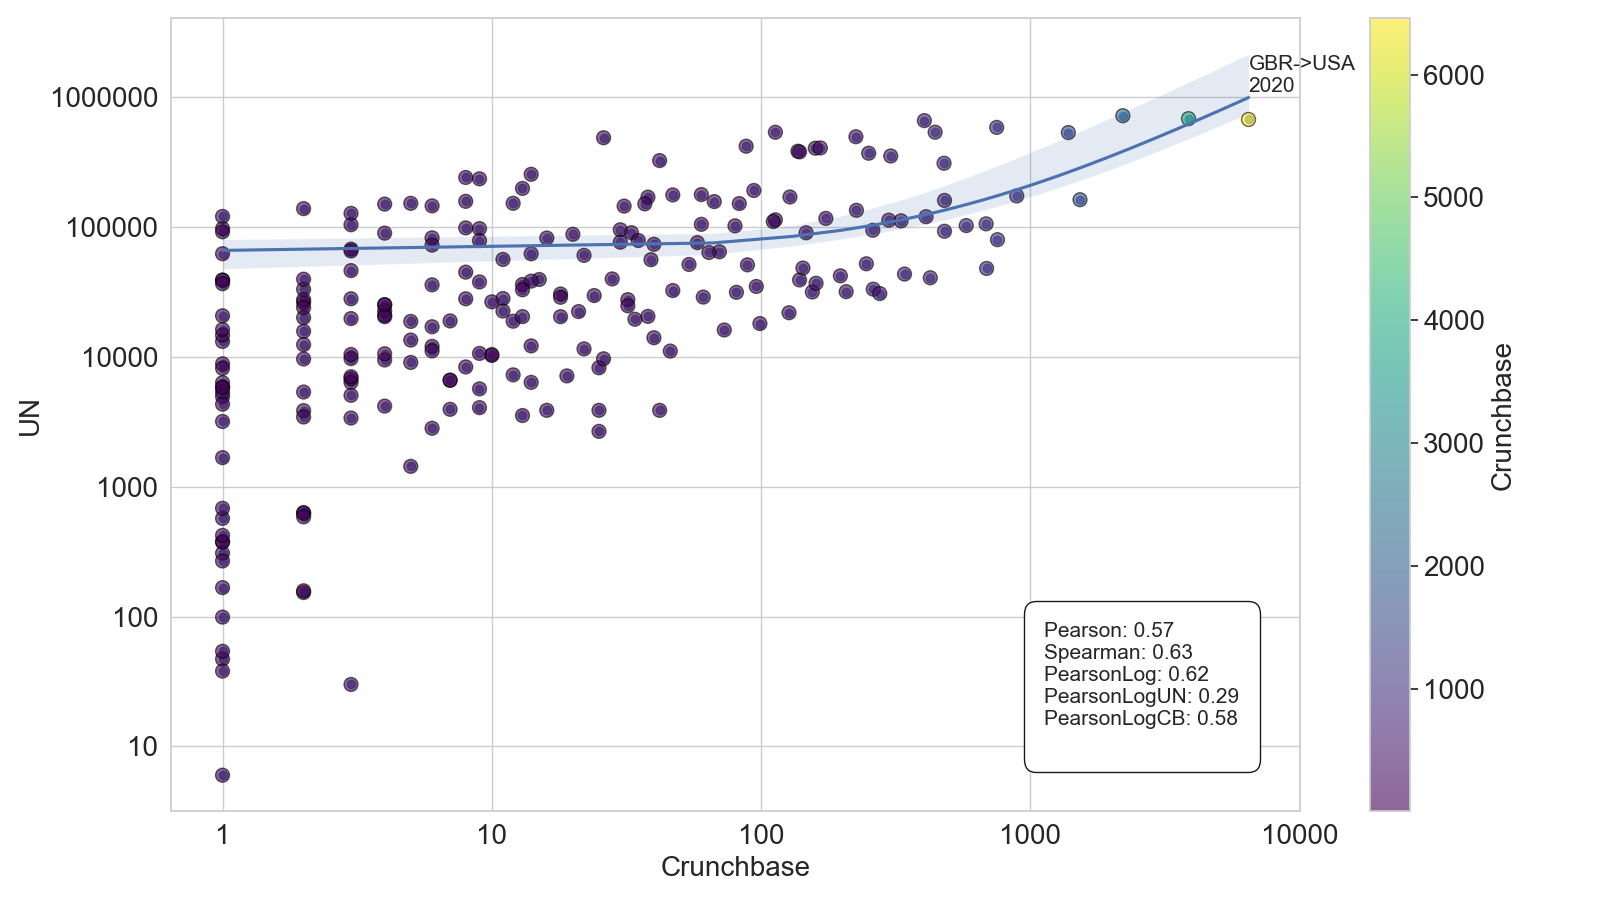
\includegraphics[width=\textwidth]{images/Migration_Stocks/NORTHAMERICA_EUROPE/Migration Stocks from Europe to North America.png}
    \caption{Scorte di migranti di nazionalità Europea in nord America (2010, 2015 e 2020).}
    \label{fig:migstockresNordAmnatEur}
  \end{minipage}
  %\hfill
  \begin{minipage}[b]{1\textwidth}
    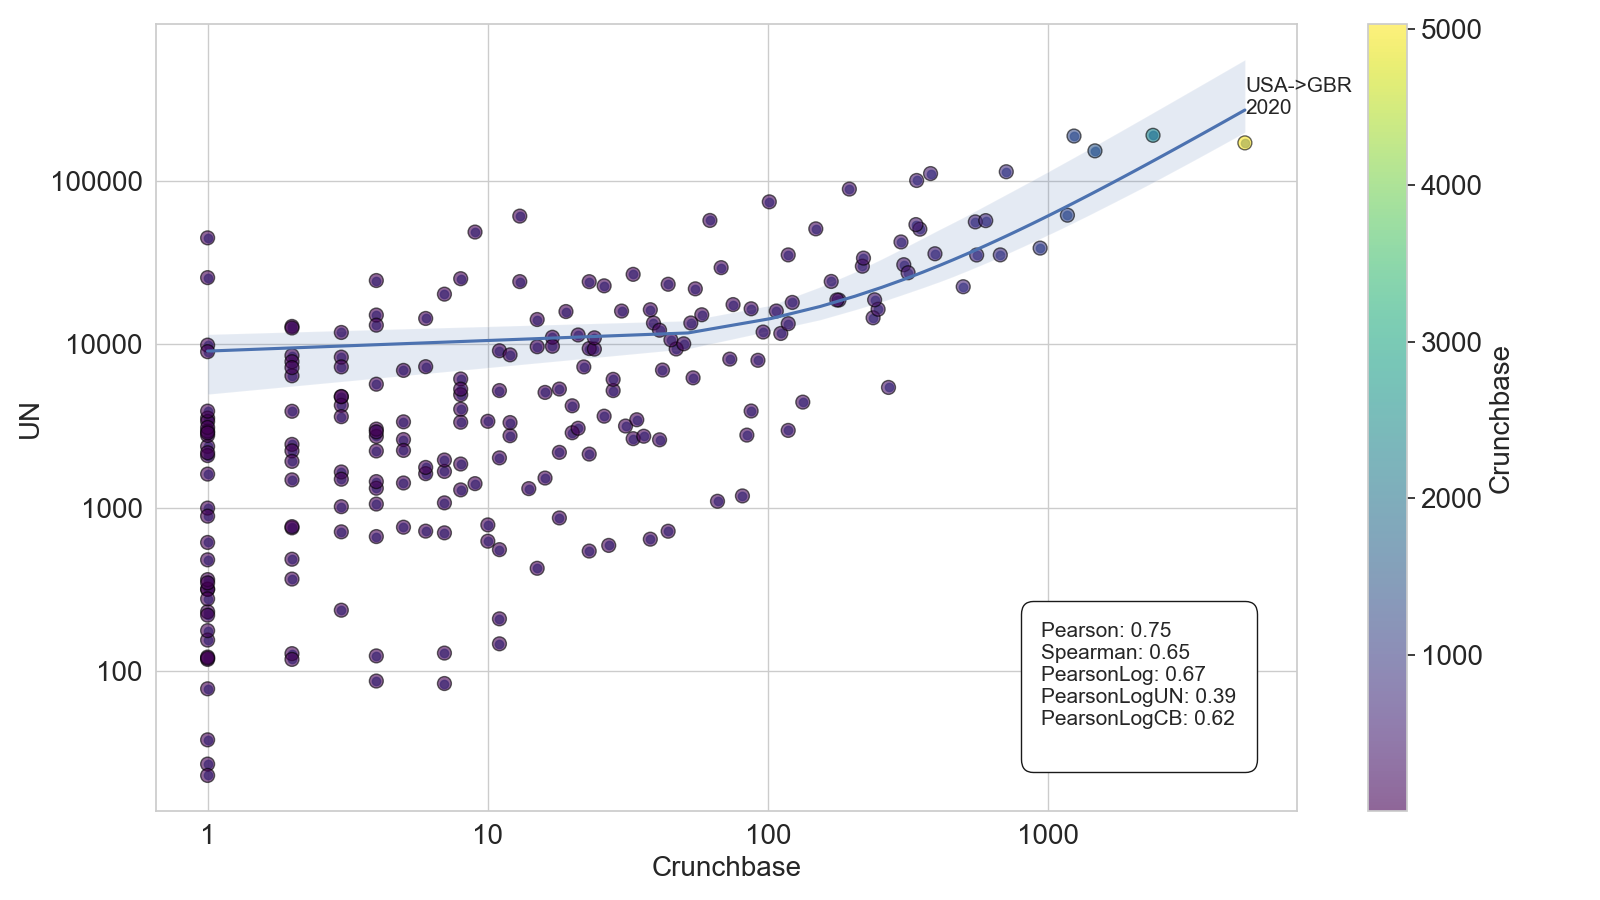
\includegraphics[width=\textwidth]{images/Migration_Stocks/NORTHAMERICA_EUROPE/Migration Stocks from North America to Europe.png}
    \caption{Scorte di migranti di nazionalità nord americana in Europa (2010, 2015 e 2020).}
    \label{fig:migstockresEuropenatNordAm}
  \end{minipage}
\end{figure}
Viene effettuato un filtro sui dati Crunchbase e UN per il continente Europa e il subcontinente nord americano. Il grafico in Figura \ref{fig:migstockresNordAmnatEur} analizza le scorte migratore di persone di nazionalità europea in nord America. Sull'asse delle x vengono posti i valori Crunchbase, sull'asse delle y i valori UN. In questo caso, la correlazione di Pearson è di 0.57 e l'indice di Spearman di 0.63. La correlazione di Pearson ponendo le scorte in scala logaritmica si eguaglia all'indice di Spearman (0.62).
Questi risultati suggeriscono quindi dei buoni livelli di correlazione. Il valore massimo di scorte di migranti altamente qualificati per Crunchbase, indicato nel grafico accanto al punto, è di britannici in nord America.
In Figura \ref{fig:migstockresEuropenatNordAm} viene mostrato il confronto delle scorte di nazionalità nord americana in Europa. 
La correlazione di Pearson è di 0.75 e l'indice di Spearman di 0,65, indicando una correlazione positiva forte per Pearson. Il valore di scorte maggiori per Crunchbase si ottiene per i migranti statunitensi in Inghilterra nel 2020.
Come già mostrato durante l'analisi dell'utenza di Crunchbase (Sezione \ref{sec:datasetcollezzionato}), Europa e Nord America sono le zone più rappresentate.
\FloatBarrier

\subsection{Discussione}
Dato che a differenza di Crunchbase, UN dispone di sole scorte quinquennali, sono stati analizzati dati relativi al 2010, 2015 e 2020
Le scorte migratorie di Crunchbase presentano una correlazione debole con UN nel caso generale (Sezione \ref{UN_stock}).
Il caso di studio dell'Italia (Sezione \ref{itastock}) mostra correlazioni discrete per gli emigrati dall'Italia, ma nessuna correlazione per gli immigrati in Italia.
Per il caso di studio della Gran Bretagna (Sezione \ref{gbrstock}) sia le scorte di emigrati che di immigrati hanno correlazione discreta con UN.
L'ultimo caso di studio si focalizza sugli stati del continente europeo e sul nord America (Sezione \ref{europenordamstock}). La correlazione è discreta per gli emigrati europei in nord America. Inoltre, Pearson indica una forte correlazione per gli immigrati nord americani in Europa. 
I risultati ottenuti suggeriscono che a seconda dei casi e soggetti di studio, i dati di Crunchbase potrebbero essere impiegati per lo studio delle scorte di migranti. 

\section{Analisi dei flussi}
\label{sec:analisi_flussi}
In questa sezione vengono analizzati flussi di migranti di Crunchbase aggregati per zona geografica.
Oltre allo studio dei flussi aggregati, per la Gran Bretagna è stato analizzato il periodo connesso alla Brexit (Sezione \ref{brexitflowscrunch}).
I flussi di Crunchbase sono stati confrontati, mediante il calcolo della correlazione di Pearson e di Spearman, con i flussi in UN, Eurostat e con l'unione dei due, per gli anni dal 2010 al 2020.
I risultati dello studio dei flussi aggregati per paesi lungo tutto l'arco temporale coperto dai dati (dal 2010 al 2020) sono stati visualizzati mediante chord diagram.
Per il caso studio relativo all'Italia è stato impiegato il solo dataset dei flussi Eurostat. Per la Gran Bretagna è stata usata l'unione dei flussi in UN ed Eurostat. 
Come per le scorte (Sezione \ref{stockCrunchbase}) la visualizzazione dei risultati avviene attraverso grafici di dispersione.
\FloatBarrier
\subsection{Dati di Crunchbase} 
\label{flowscrunch}

\begin{figure}[tbp]
    \begin{subfigure}{0.48\textwidth}
        %\raggedleft         
        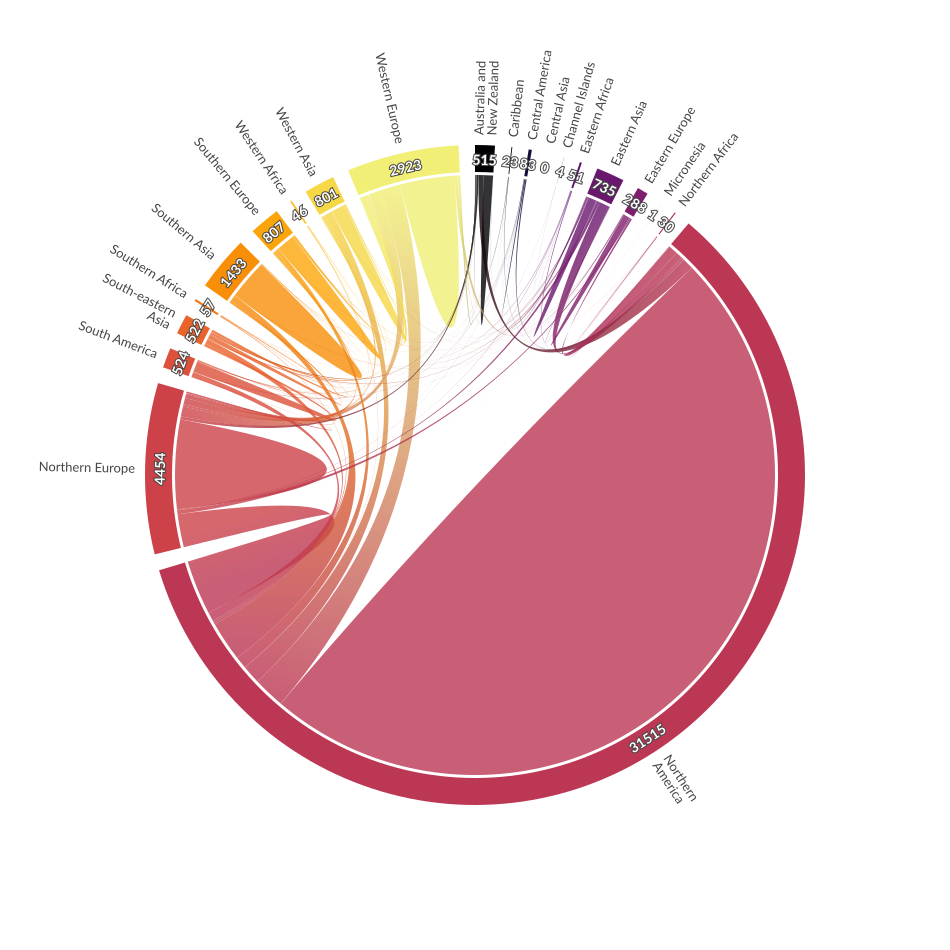
\includegraphics[scale=0.34]{images/SVG/Chords/Crunchbase/Crunchbase_Cit_Red.png}
        \caption{Flussi di cittadini}
        \label{fig:chordCrunchbase_cit}
    \end{subfigure}
    \begin{subfigure}{0.48\textwidth}
        %\raggedleft         
        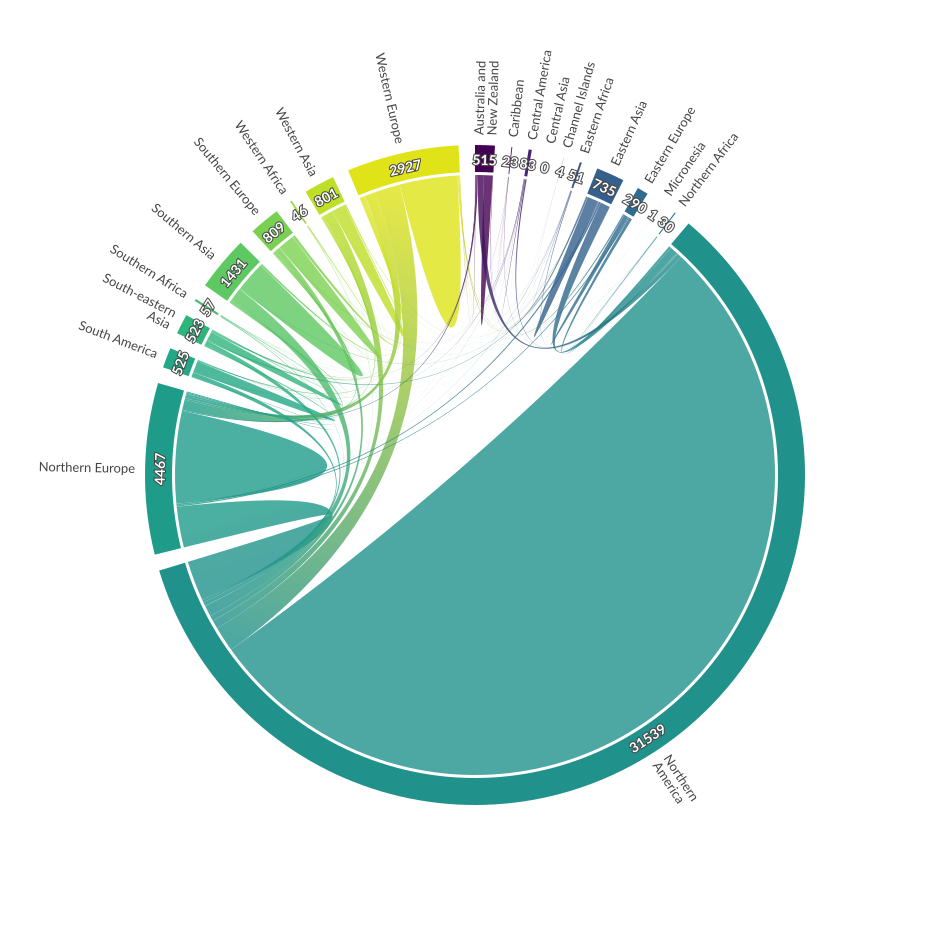
\includegraphics[scale=0.34]{images/SVG/Chords/Crunchbase/Crunchbase_Res_Blue.png}
        \caption{Flussi di residenti}
        \label{fig:chordCrunchbase_res}
    \end{subfigure}
    \caption{Flussi di migranti da Crunchbase aggregati per zone geografiche, dal 2010 al 2020. Il numero relativo alla zona indica il numero di flussi uscenti.}
    \label{fig:chordCrunchbase}
\end{figure}

I flussi in Figura \ref{fig:chordCrunchbase_cit} relativi a tutti i cittadini (utenti che sono residenti nello stato della nazionalità) presenti su Crunchbase sono maggiori per il nord America, il nord Europa e l'Europa dell'ovest. 
Buona parte dei flussi sono rappresentati da persone che si spostano in paesi della stessa zona, in particolare per il nord America. \par

La Figura \ref{fig:chordCrunchbase_res} rappresenta i flussi migratori dei residenti osservabili dai dati di Crunchbase. 
I flussi dei residenti sono simili a quelli dei cittadini (Sezione \ref{flowscrunch}). I flussi del nord America si presentano, anche in questo caso, i più numerosi. 

%Questo suggerisce che gli utenti su Crunchbase che migrano siano sia cittadini che residenti nello stato di provenienza. 
Inoltre, i risultati mostrano che la distribuzione dei flussi migratori su Crunchbase è maggiore per il subcontinente nord americano e per l'Europa. Tuttavia, sono presenti flussi relativi anche agli altri sub-continenti, sebbene siano minori. 
\FloatBarrier

\subsubsection{Caso di studio: Gran Bretagna e la Brexit}
\label{brexitflowscrunch}


\begin{figure}[!h]
    \centering
    \begin{subfigure}{0.47\textwidth}
        \raggedleft         
        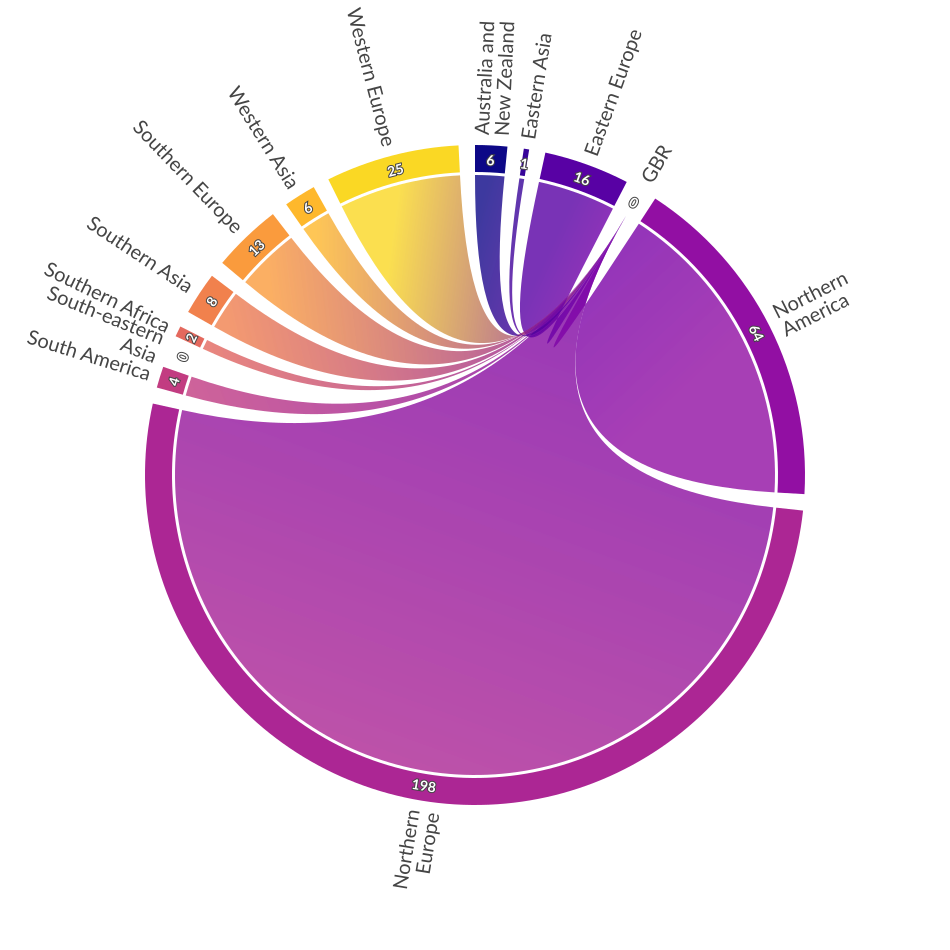
\includegraphics[scale=0.34]{images/SVG/Chords/Brexit/togbrflows_2015.png}
        \caption{Flussi 2015}
        \label{fig:togbr_flowsBrexit2015}
    \end{subfigure}
    \begin{subfigure}{0.47\textwidth}
        \raggedleft         
        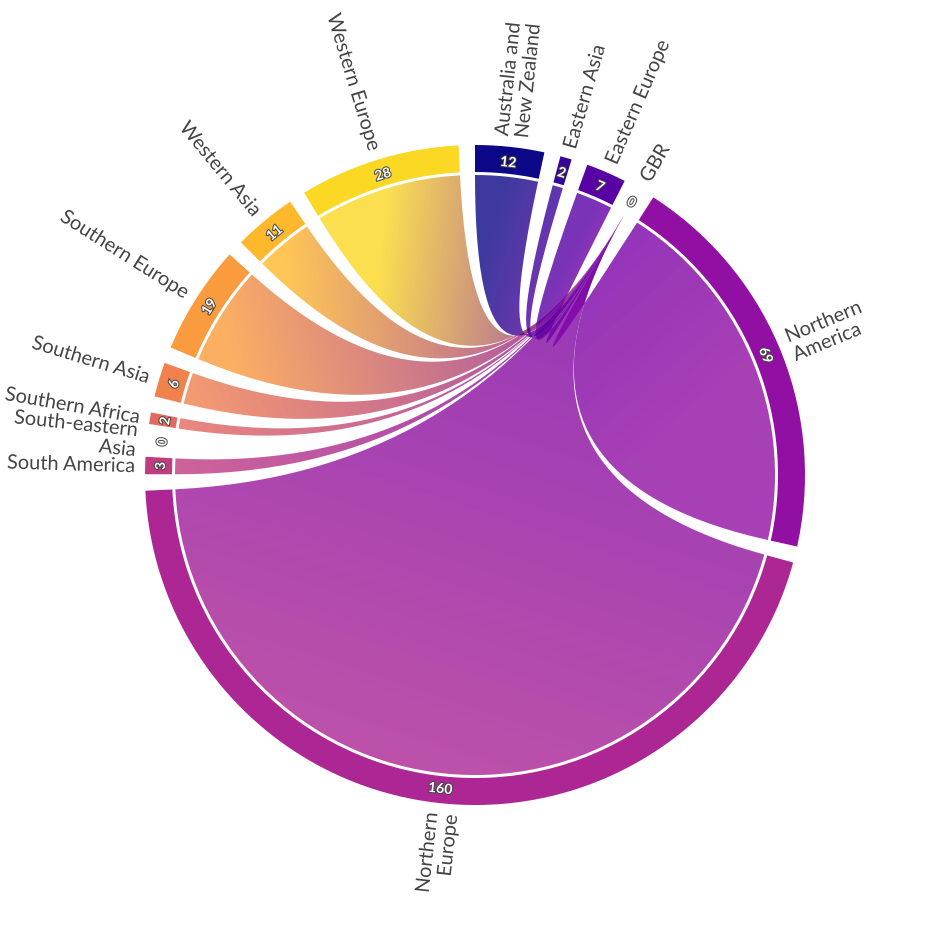
\includegraphics[scale=0.34]{images/SVG/Chords/Brexit/togbrflows_2017.png}
        \caption{Flussi 2017}
        \label{fig:togbr_flowsBrexit2017}
    \end{subfigure}
    \caption{Flussi di immigrati in Gran Bretagna da Crunchbase, per gli anni 2015 e 2017.}
    \label{fig:togbr_flowsBrexit}
\end{figure}


La Figura \ref{fig:togbr_flowsBrexit2015} mostra i flussi di immigrati, in Crunchbase, che interessano la Gran Bretagna nell'anno 2015. Gli stati vengono aggregati per zona, il numero relativo alla zona indica il numero di flussi uscenti. I flussi di emigrati dalla Gran Bretagna sono stati ignorati lasciando spazio ai flussi di immigrati nel grafico. I flussi maggiori provengono dal nord Europa, il nord America e l'Europa dell'ovest. 
La Figura \ref{fig:togbr_flowsBrexit2017} mostra i flussi di migranti, da Crunchbase, verso la Gran Bretagna nel 2017. La Figura mostra leggere differenze nei flussi rispetto al 2015. I flussi provenienti dal nord Europa sono diminuiti di circa il 20\% (da 198 a 160). 
Al contrario, sono aumentati i flussi verso l'Australia e la Nuova Zelanda (da 6 a 12), e verso il sud Europa (da 13 a 18). Il nord America ha avuto una variazione di sole 5 persone, da 64 a 69. 

I risultati ottenuti mostrano che il nord America, il nord Europa e l'ovest Europa sono le zone geografiche più coinvolte nei flussi di migrazione di utenti altamente qualificati. Queste osservazioni sono in linea con quanto osservato nello studio dell'utenza Crunchbase (Sezione \ref{sec:datasetcollezzionato}) e nell'analisi delle scorte (Sezione \ref{stockCrunchbase}).

\FloatBarrier
\subsection{Confronto Crunchbase con UN ed Eurostat} 
Come per i dati delle scorte, l'insieme dei dati relativi ai flussi di Crunchbase viene intersecato con quelli dei flussi presenti negli altri dataset. 
Per il confronto con UN, i flussi Crunchbase vedono una riduzione fino a 5.532 combinazioni (-1184). Per il confronto con Eurostat la diminuzione dei dati è nettamente superiore, arrivando a 2.208 combinazioni (-4508). Ogni combinazione fa riferimento sia al caso di cittadini che al caso di residenti.

\paragraph{Eurostat} 
\label{ESTAT_original}

\begin{figure}[ht]
    \centering
    \begin{subfigure}{\textwidth}
        \centering
        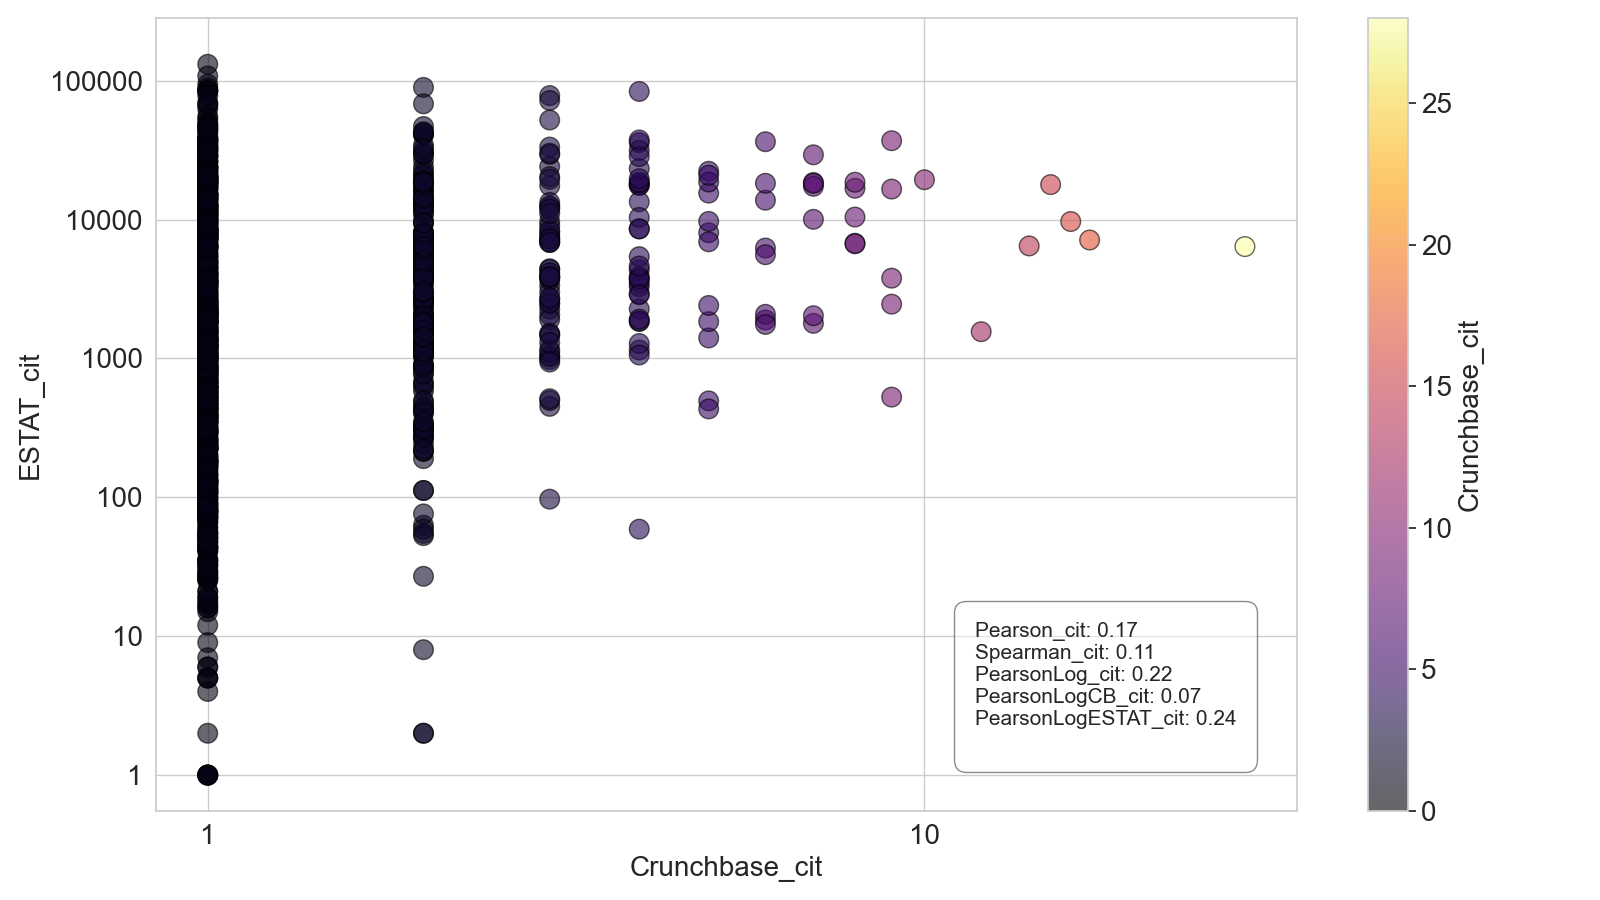
\includegraphics[width=1.0\textwidth]{images/flows/original/ESTAT_cit_False.png}
        \caption{Flussi cittadini}
        \label{fig:estatcrunchfalse_cit}
    \end{subfigure}
    \begin{subfigure}{\textwidth}
        \centering
        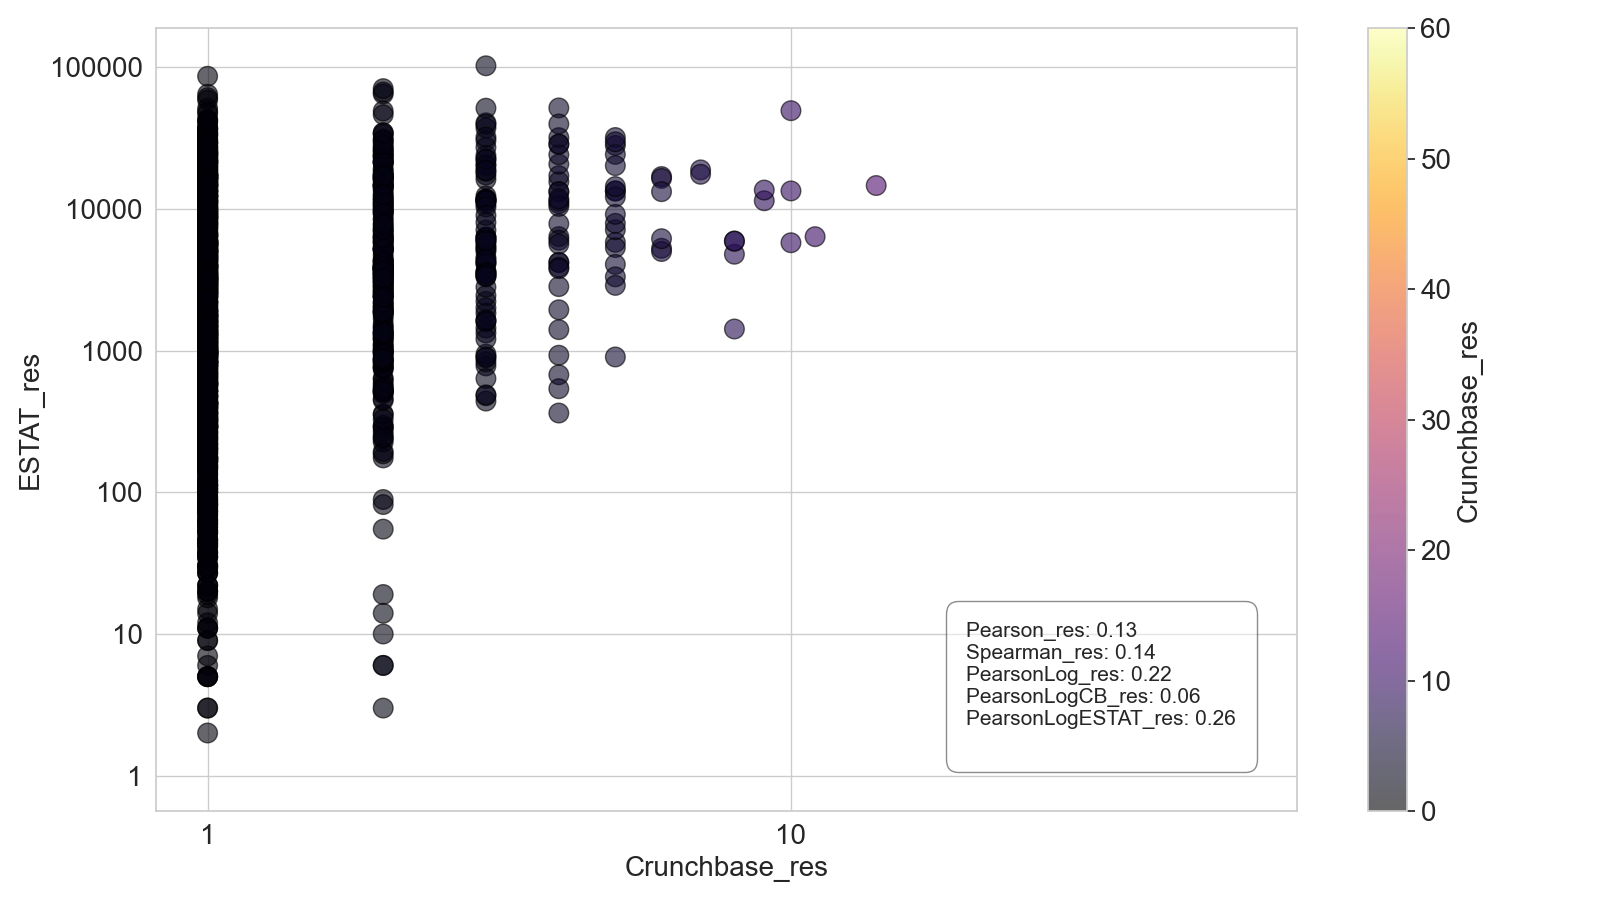
\includegraphics[width=1.0\textwidth]{images/flows/original/ESTAT_res_False.png}
        \caption{Flussi residenti}
        \label{fig:estatcrunchfalse_res}
    \end{subfigure}
    \caption{Confronto dei flussi Crunchbase con i flussi Eurostat (2010 al 2020).}
    \label{fig:estatcrunchfalse}
\end{figure}
\par 
La Figura \ref{fig:estatcrunchfalse_cit} mostra il confronto tra i flussi di Crunchbase ed di Eurostat per i cittadini che migrano dal paese di nazionalità. La correlazione di Pearson è di 0.17, simile all'indice di Spearman (0.11), indicando una scarsa relazione fra i due set di dati.
Il grafico in Figura \ref{fig:estatcrunchfalse_res} presenta i flussi dei residenti emigranti in Crunchbase e in  Eurostat. Sebbene ci sia un incremento del valore massimo di migranti rispetto al caso dei cittadini, le correlazioni sono molto basse (Pearson 0.13, Spearman 0.14). 
\paragraph{UN}
\label{UN_original}

\begin{figure}[tb]
    \centering
    \begin{subfigure}{\textwidth}
        \centering
        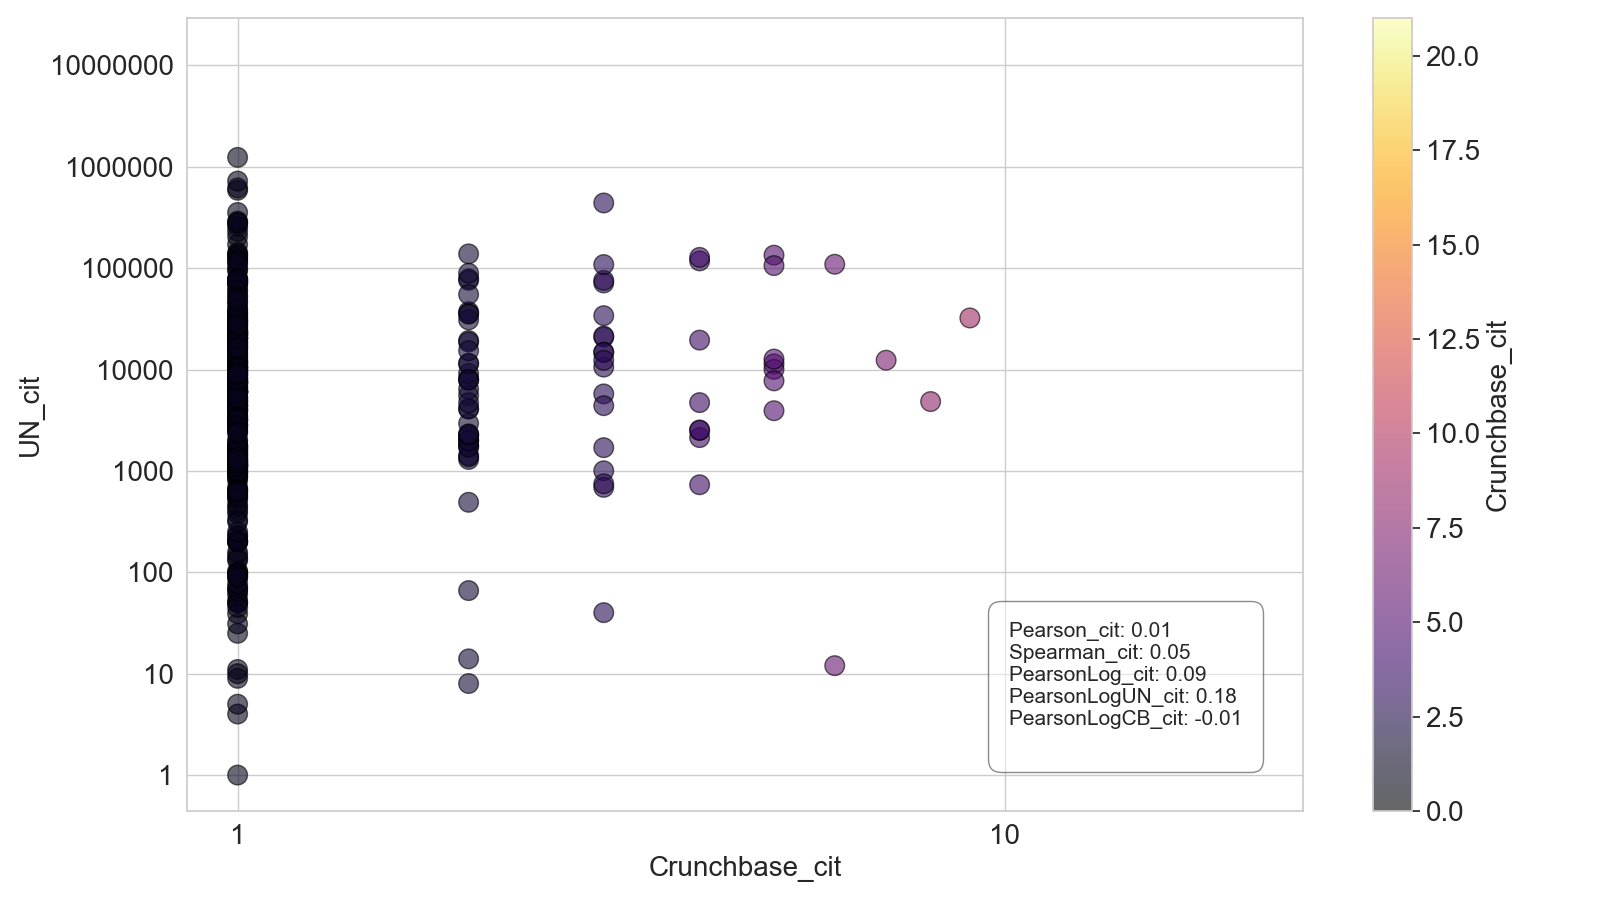
\includegraphics[width=1.0\textwidth]{images/flows/original/UN_cit_False.png}
        \caption{Flussi cittadini}
        \label{fig:uncrunchfalse_cit}
    \end{subfigure}
    \begin{subfigure}{\textwidth}
        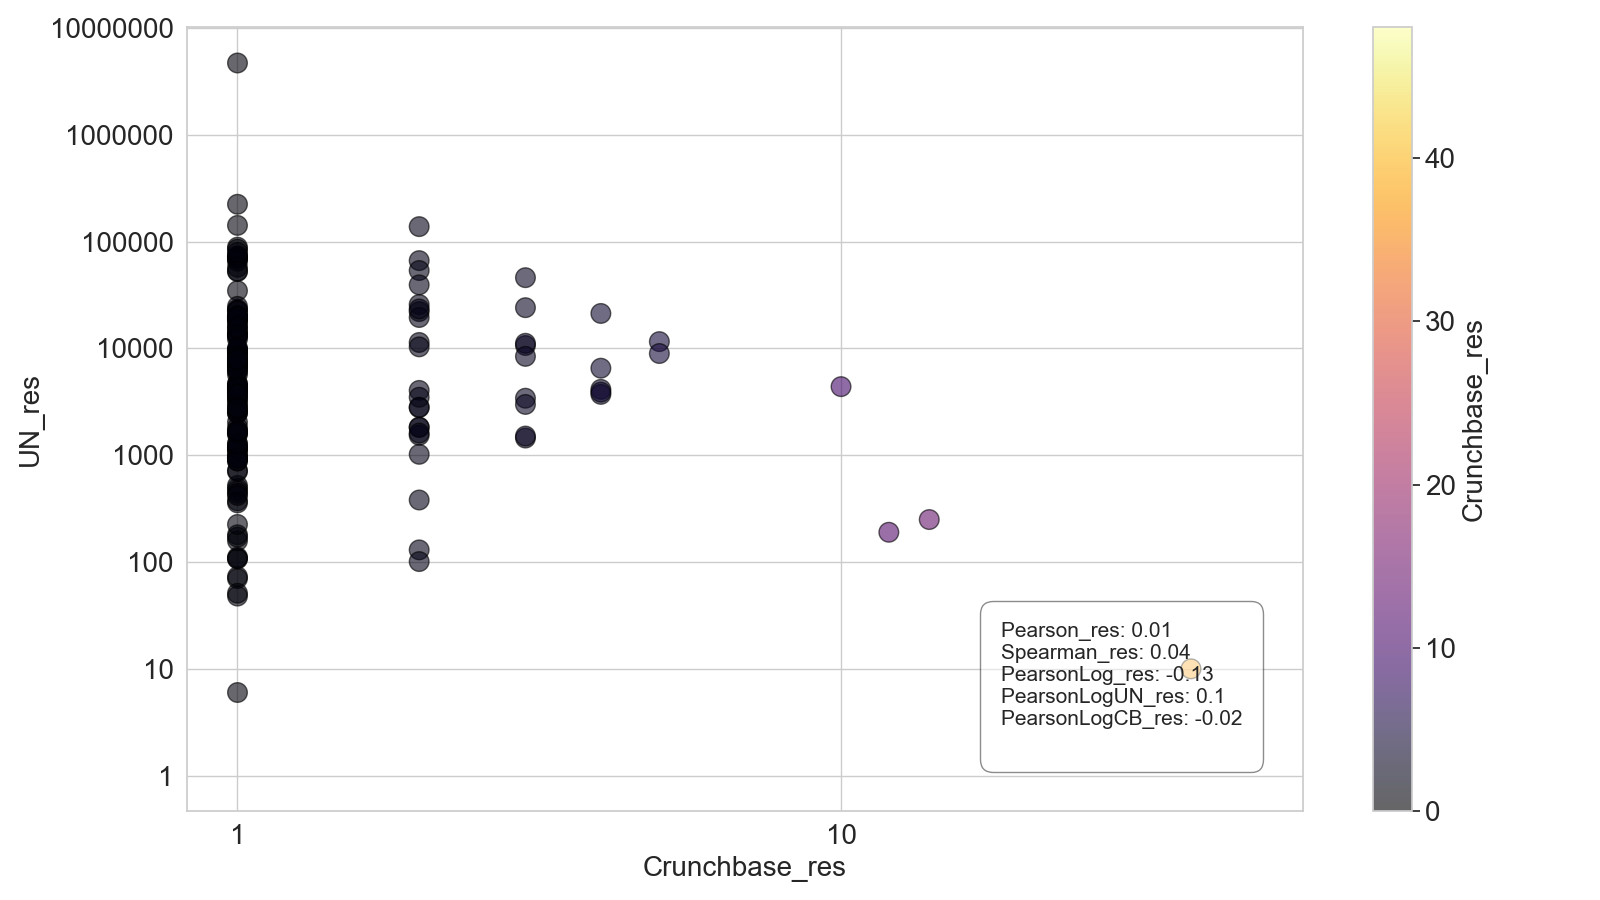
\includegraphics[width=1.0\textwidth]{images/flows/original/UN_res_False.png}
        \caption{Flussi residenti}
        \label{fig:uncrunchfalse_res}
    \end{subfigure}
    \caption{Confronto dei flussi in Crunchbase con UN dal 2010 al 2020.}
    \label{fig:uncrunchfalse}
\end{figure}
La Figura \ref{fig:uncrunchfalse_cit} mostra i flussi dei cittadini che hanno migrato in confronto a UN. La Figura \ref{fig:uncrunchfalse_res} mostra i flussi dei residenti. Entrambi i casi non presentano correlazione per Pearson e Spearman. Il valore massimo di flussi di migranti per Crunchbase in confronto a UN non supera le 40 unità. 
Il confronto dei dati relativi ai flussi di Crunchbase con i flussi di UN (Sezione \ref{UN_original}) ed i flussi di Eurostat (Sezione \ref{ESTAT_original}) non ha mostrato correlazioni significative.
\FloatBarrier

\subsection{Confronto UN ed Eurostat con stati aggregati}
\paragraph{Eurostat con stati aggregati}
Analizziamo i flussi Crunchbase aggregando (sommando) i flussi degli stati per zone geografiche.
L'analisi di dati aggregati porta ad avere informazioni meno specifiche per gli stati in dettaglio, ma permette di comprendere quali sono le zone più interessate dai flussi in ingresso ed in uscita.
\label{ESTAT_aggregated}
\begin{figure}[!ht]
    \centering
    \begin{subfigure}{\textwidth}
        \centering
        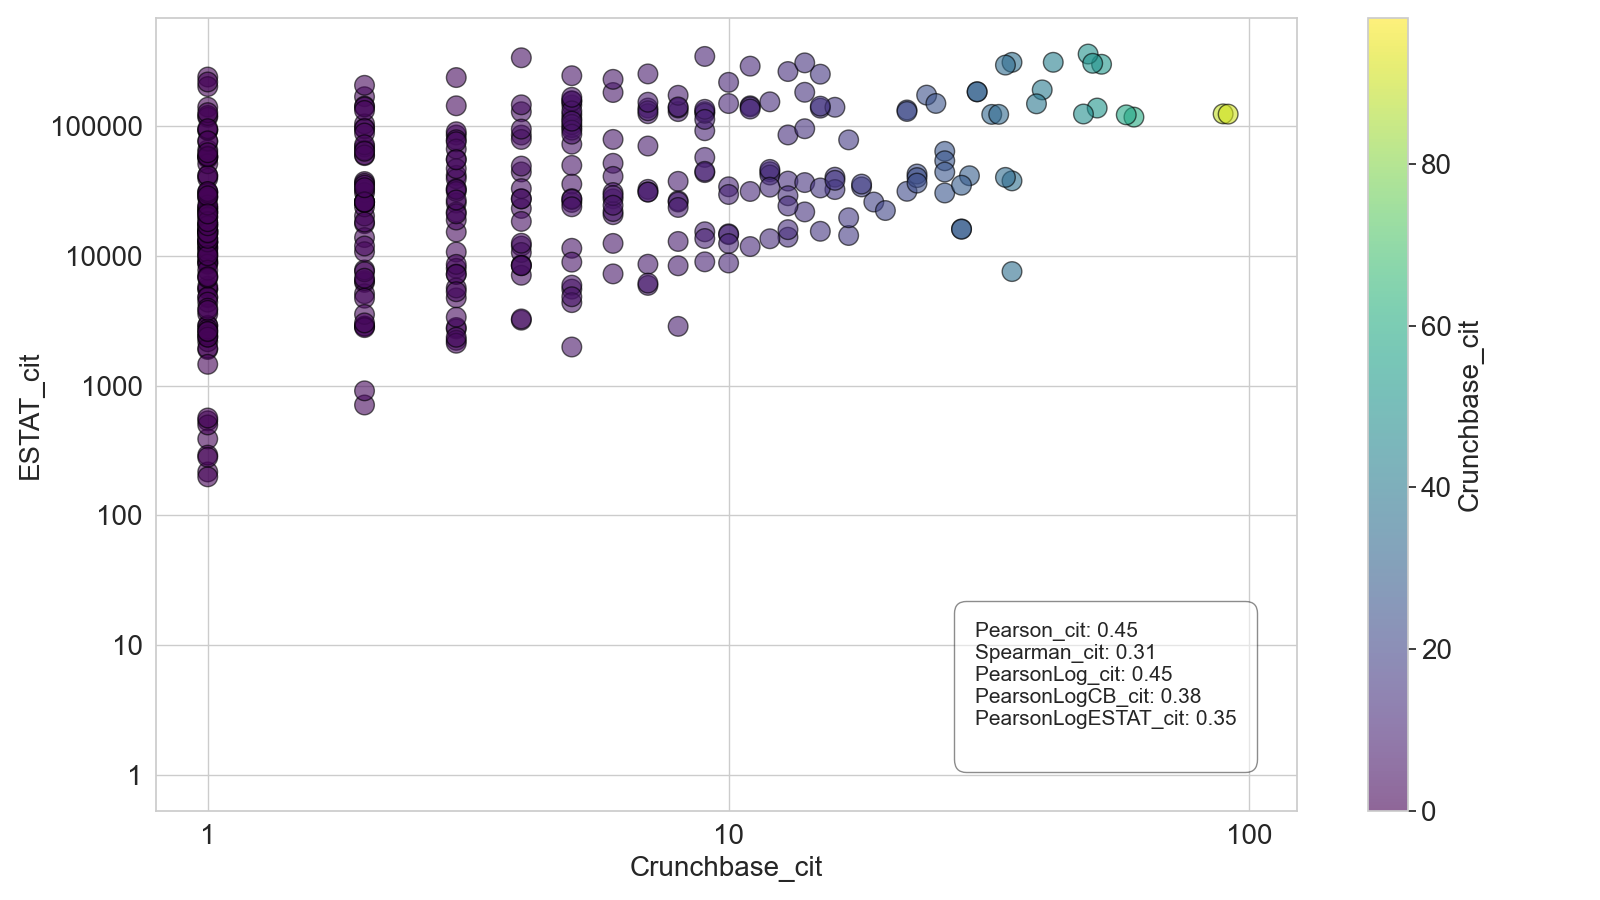
\includegraphics[width=0.95\textwidth]{images/flows/aggregated/ESTAT_cit_True.png}
        \caption{Flussi cittadini}
        \label{fig:estatcrunchtrue_cit}
    \end{subfigure}
    \begin{subfigure}{\textwidth}
        \centering
        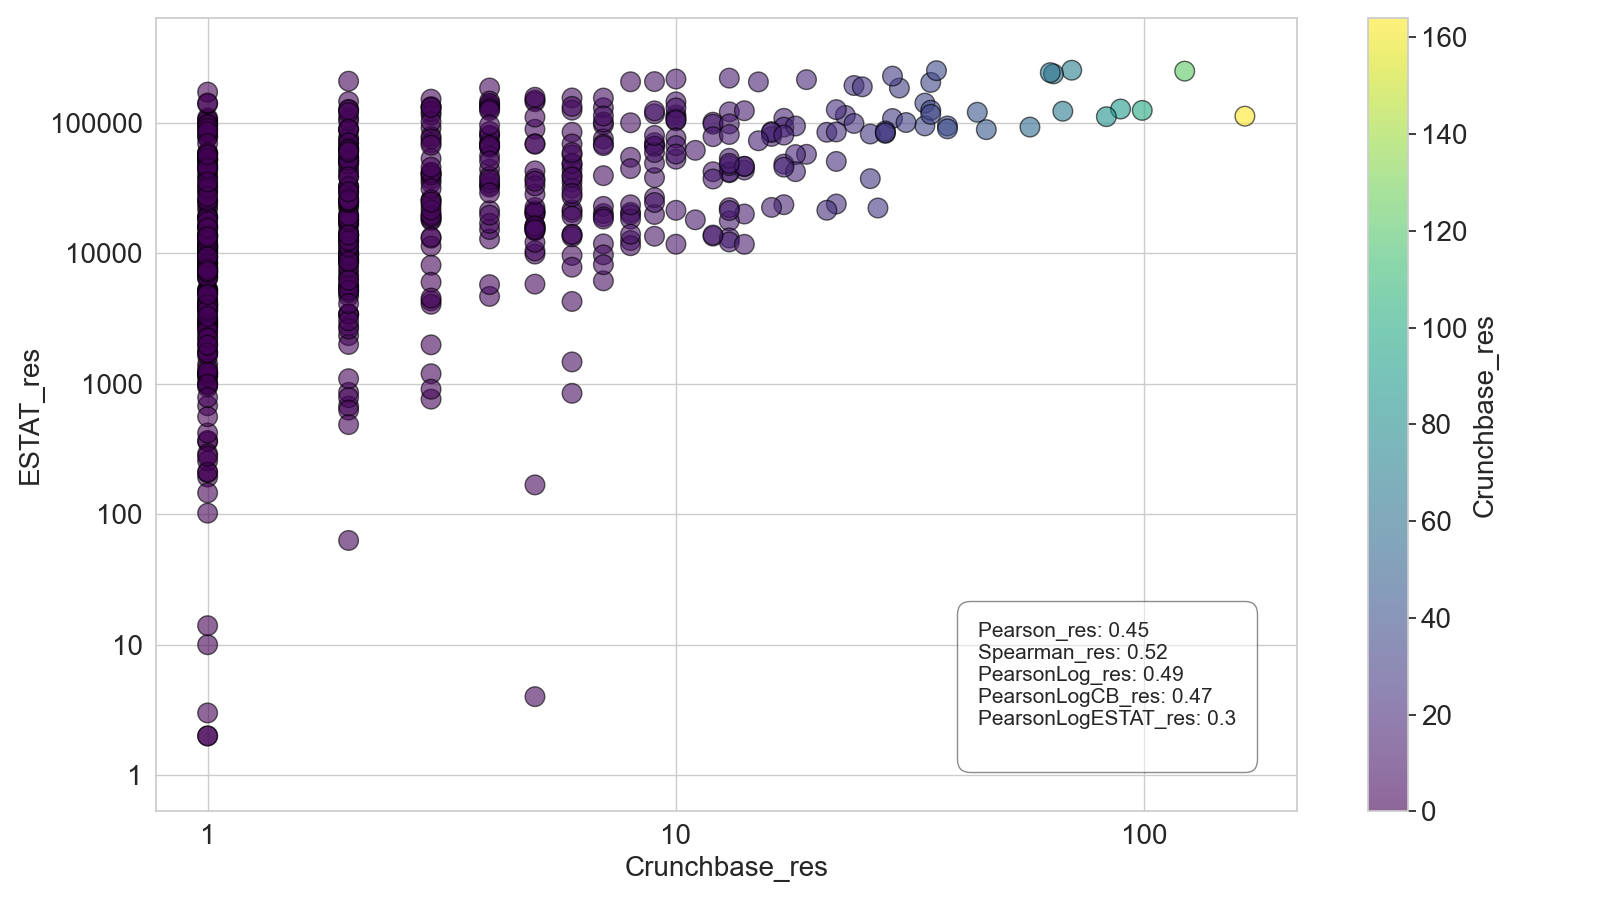
\includegraphics[width=0.95\textwidth]{images/flows/aggregated/ESTAT_res_True.png}
        \caption{Flussi residenti}
        \label{fig:estatcrunchtrue_res}
    \end{subfigure}
    \caption{Confronto dei flussi Crunchbase con i flussi in Eurostat aggregati per zone geografiche dal 2010 al 2020}
    \label{fig:estatcrunchtrue}
\end{figure}
Nella Figura \ref{fig:estatcrunchtrue_cit} viene mostrato il grafico di confronto tra Eurostat e Crunchbase dei cittadini emigrati aggregati per zone geografiche, dal 2010 al 2020.
La correlazione di Pearson è di 0.45, a differenza dell'indice di Spearman che indica un valore di 0.31. Il coefficiente  di Pearson suggerisce che esista una correlazione debole tra i dati dei flussi aggregati di Crunchbase e UN.


La Figura \ref{fig:estatcrunchtrue_res} mostra il confronto tra Eurostat e Crunchbase dei residenti migrati aggregati per zone geografiche. La correlazione di Pearson (0.45) indica una correlazione debole, l'indice di Spearman (0.52) invece indica una correlazione discreta. La correlazione di Pearson calcolata con i flussi Crunchbase in scala logaritmica ottiene un valore superiore (0.47) alla correlazione normale, ma pur sempre basso.

\paragraph{UN con stati aggregati}
\label{UN_aggregated}
\begin{figure}[tb]
    \centering
    \begin{subfigure}{\textwidth}
        \centering
        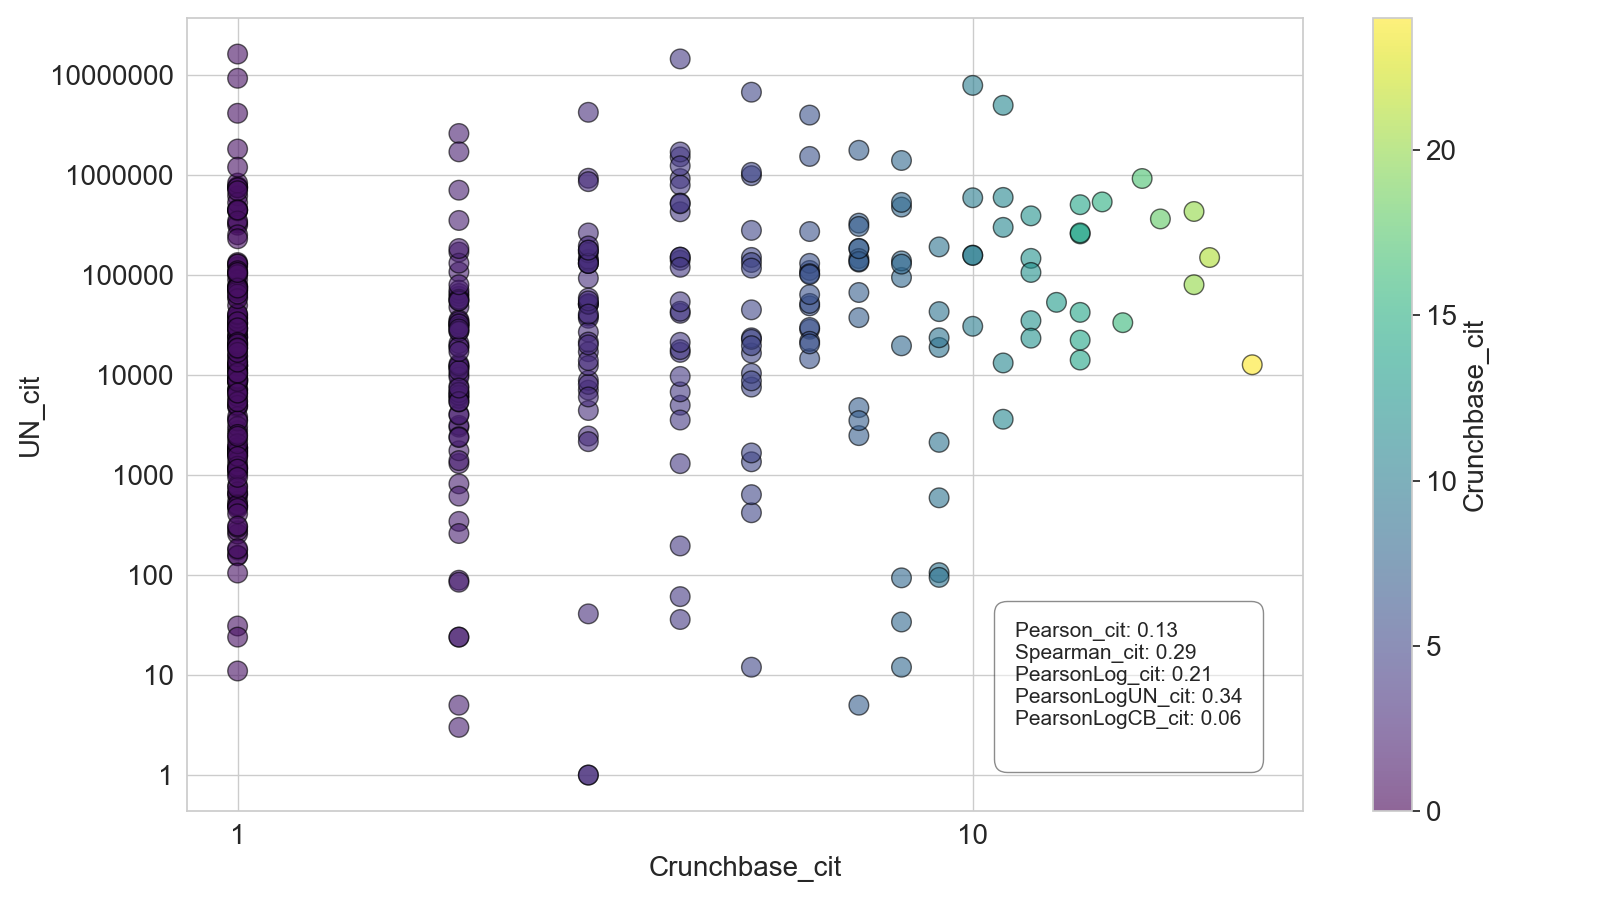
\includegraphics[width=0.95\textwidth]{images/flows/aggregated/UN_cit_True.png}
        \caption{Flussi cittadini}
        \label{fig:uncrunchtrue_cit}
    \end{subfigure}
    \begin{subfigure}{\textwidth}
        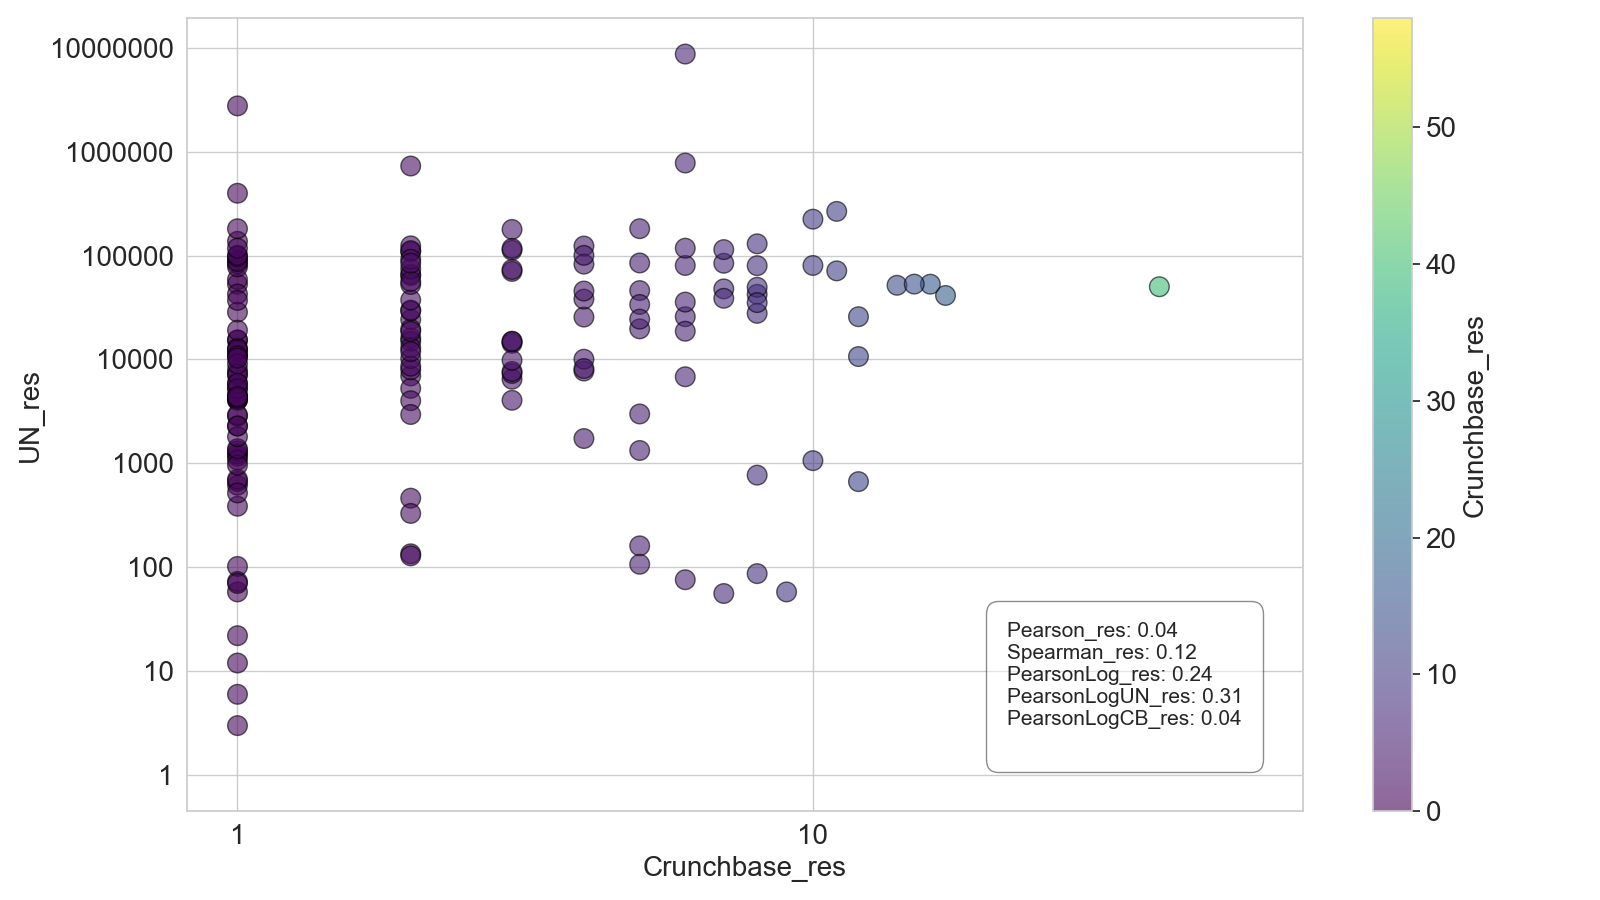
\includegraphics[width=0.95\textwidth]{images/flows/aggregated/UN_res_True.png}
        \caption{Flussi residenti}
        \label{fig:uncrunchtrue_res}
    \end{subfigure}
    \caption{Confronto dei flussi Crunchbase con i flussi in UN aggregati per zone geografiche dal 2010 al 2020.}
    \label{fig:uncrunchtrue}
\end{figure}
In Figura \ref{fig:uncrunchtrue_cit} vengono mostrati i flussi dei cittadini aggregati per zone geografiche in UN e Crunchbase. Il confronto presenta una correlazione di Pearson di 0.13 ed un indice di Spearman di 0.29. Il valore della correlazione di Pearson è di 0.34 utilizzando una scala logaritmica per i soli flussi dei cittadini in UN. 
Nella Figura \ref{fig:uncrunchtrue_res} sono presenti i flussi dei residenti aggregati per zone geografiche in UN e Crunchbase. La correlazione di Pearson ha un valore di 0.04 e l'indice di Spearman è di 0.12.
I flussi migratori di UN sono più significativi per il sudest asiatico, come visto in \cite{MIMIDOC}. Come vediamo nell'analisi del flussi di Crunchbase (Sezione \ref{flowscrunch}), il sudest asiatico non è rappresentato.
Nel caso dei cittadini i risultati indicano una correlazione bassa ponendo i dati Crunchbase in scala logaritmica. Di contro, i risultati ottenuti per il confronto dei residenti indicano che non ci sia correlazione.

\FloatBarrier
\subsection{Flussi aggregati UN unito Eurostat}
\label{UNunionEstatflows}
Per questo studio i dati di Crunchbase sono stati confrontati con l'unione di UN ed Eurostat, aggregando gli stati per zona geografica. Per l'unione dei due dataset (UN e Eurostat) è stato selezionato, per ogni paese, il flusso di maggior valore tra i due insiemi. Il periodo è come negli altri casi di studio dal 2010 al 2020.
Il grafico nella Figura \ref{fig:off_true_cit} rappresenta i cittadini. La correlazione di Pearson è di 0.06, mentre l'indice di Spearman è di 0.38. Con i dati ufficiali in scala logaritmica si ha una correlazione di Pearson di 0.24. I valori del coefficiente di Pearson indicano che non sia presente correlazione, a differenza dell'indice di Spearman che determina una correlazione debole.
Nella Figura \ref{fig:off_true_res} riferita ai residenti si ottiene una correlazione di Pearson di 0.08 e un indice di Spearman di 0.37. Con i dati ufficiali in scala logaritmica si ha una correlazione di Pearson di 0.27. Come per i cittadini questo confronto ha correlazione debole per Spearman. Inoltre, i valori ottenuti sono inferiori rispetto all'analisi effettuata con i soli dati Eurostat aggregati (Sezione \ref{ESTAT_aggregated}). 

\begin{figure}[ht]
    \begin{subfigure}{\textwidth}
        \centering
        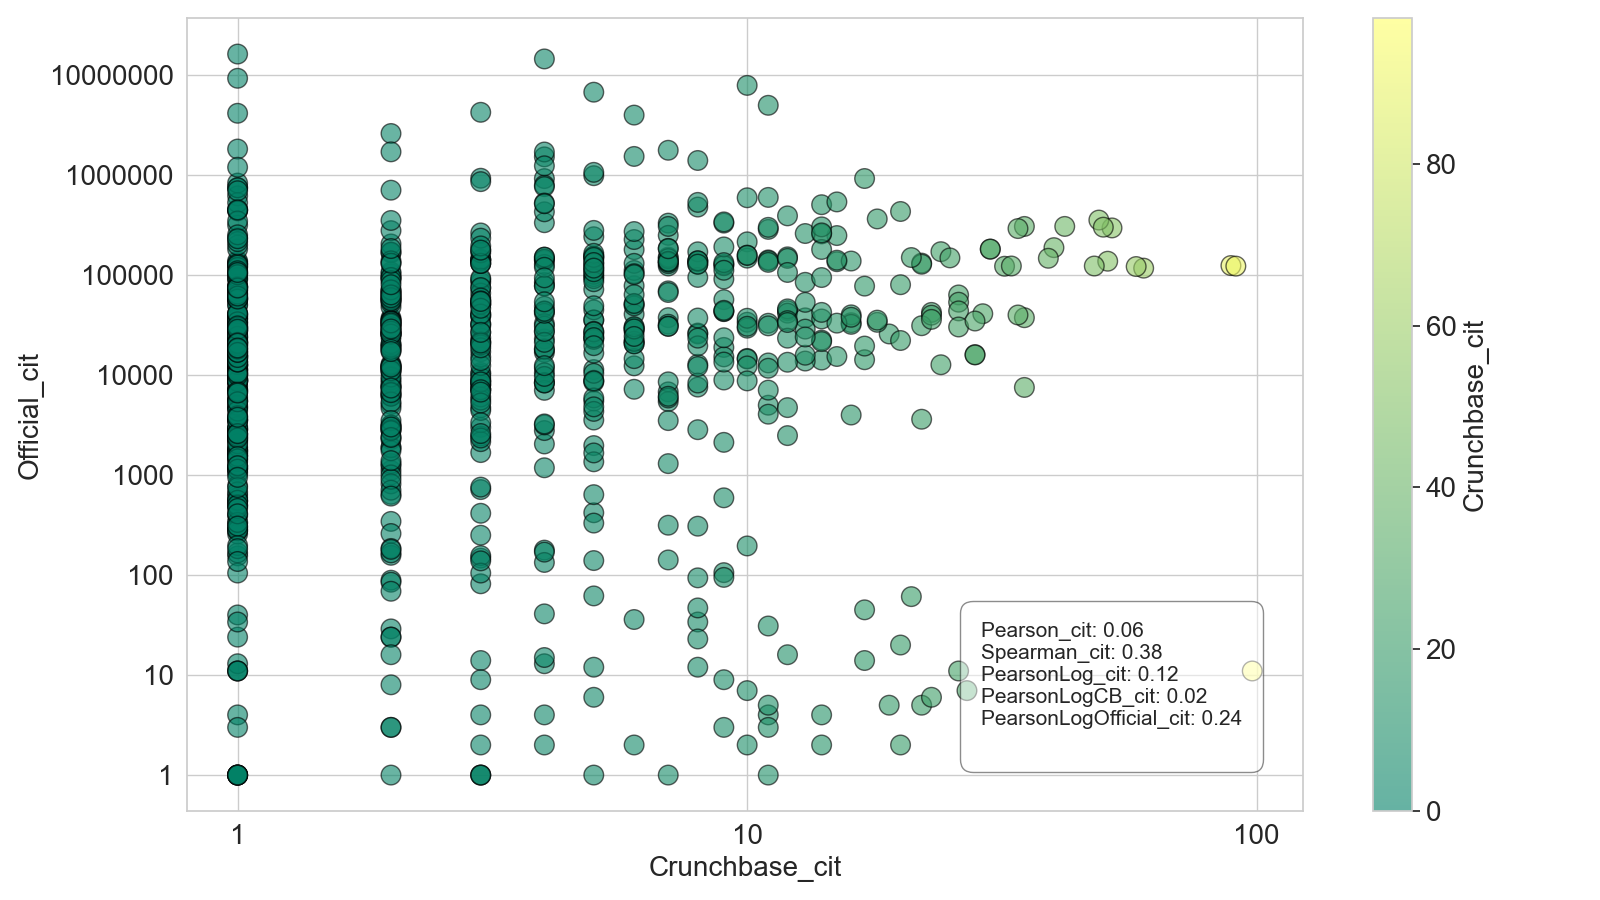
\includegraphics[width=1\textwidth]{images/congiunti/Flows/Official_cit_True.png}
        \caption{Flussi cittadini \(UN\cup{Eurostat}\)}
        \label{fig:off_true_cit}
    \end{subfigure}
\end{figure}
\begin{figure}[tb]\ContinuedFloat
    \begin{subfigure}{\textwidth}
        \centering
        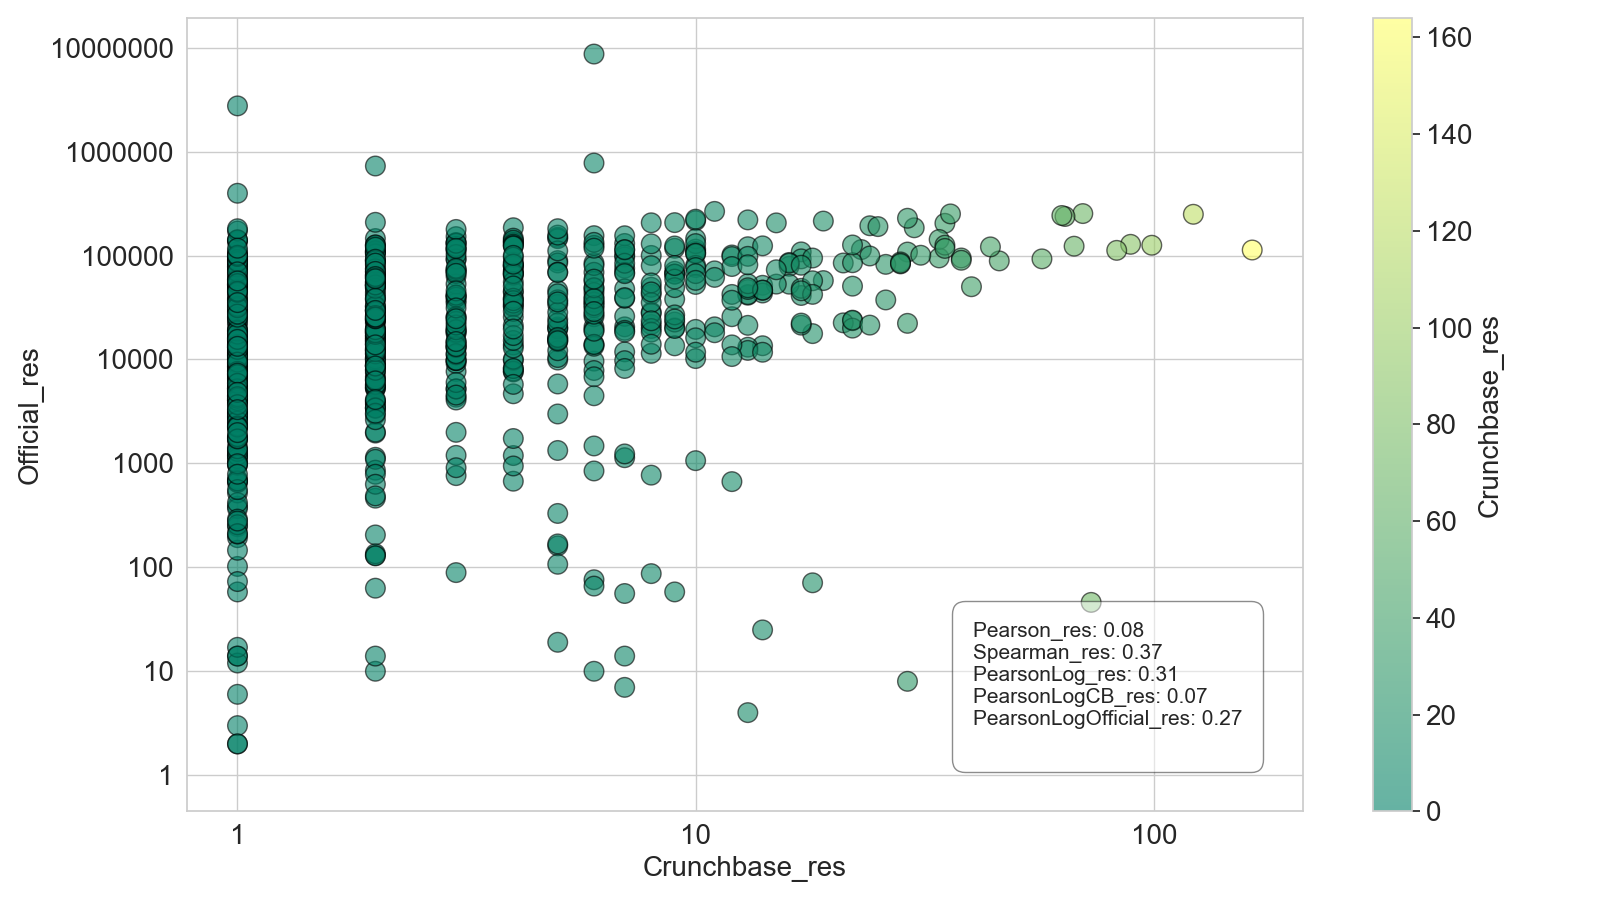
\includegraphics[width=1\textwidth]{images/congiunti/Flows/Official_res_True.png}
        \caption{Flussi residenti \(UN\cup{Eurostat}\)}
        \label{fig:off_true_res}
    \end{subfigure}
    \caption{Confronto dei flussi Crunchbase con i flussi presenti nell'unione di UN ed ESTAT (stati aggregati per zone geografiche dal 2010 al 2020.}
    \label{fig:off_true}
\end{figure}

\FloatBarrier

\subsection{Caso di studio: Italia}
In questa sezione vengono analizzati i flussi d'immigrazione ed emigrazione, di residenti e cittadini, che interessano l'Italia. Il periodo dell'analisi è riferito al periodo dell'insieme di dati collezionati (dal 2010 al 2020), ed il dataset di confronto è quello Eurostat.
\paragraph{Flussi di emigranti dall'Italia}
\label{ita_flows}
\begin{figure}[tb]
    \centering
    \begin{subfigure}{\textwidth}
        \centering
        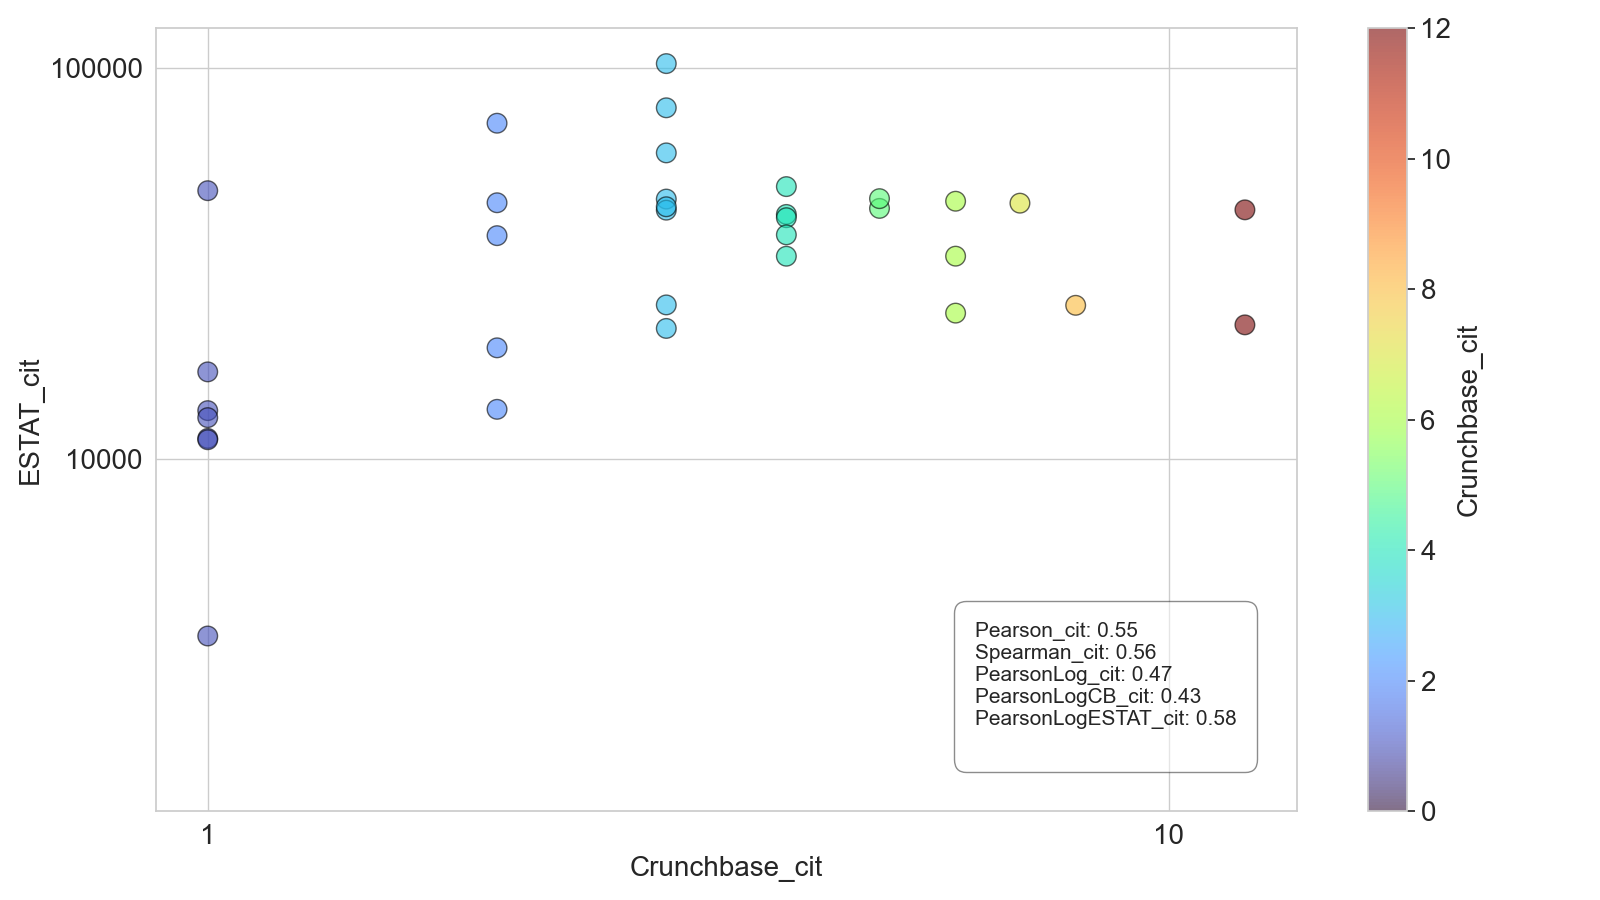
\includegraphics[width=1.0\textwidth]{images/flows/aggregated/filtered_nationality/ita/ESTAT_cit_True.png}
        \caption{Flussi cittadini}
        \label{fig:italia_nat_true}
    \end{subfigure}
    \begin{subfigure}{\textwidth}
        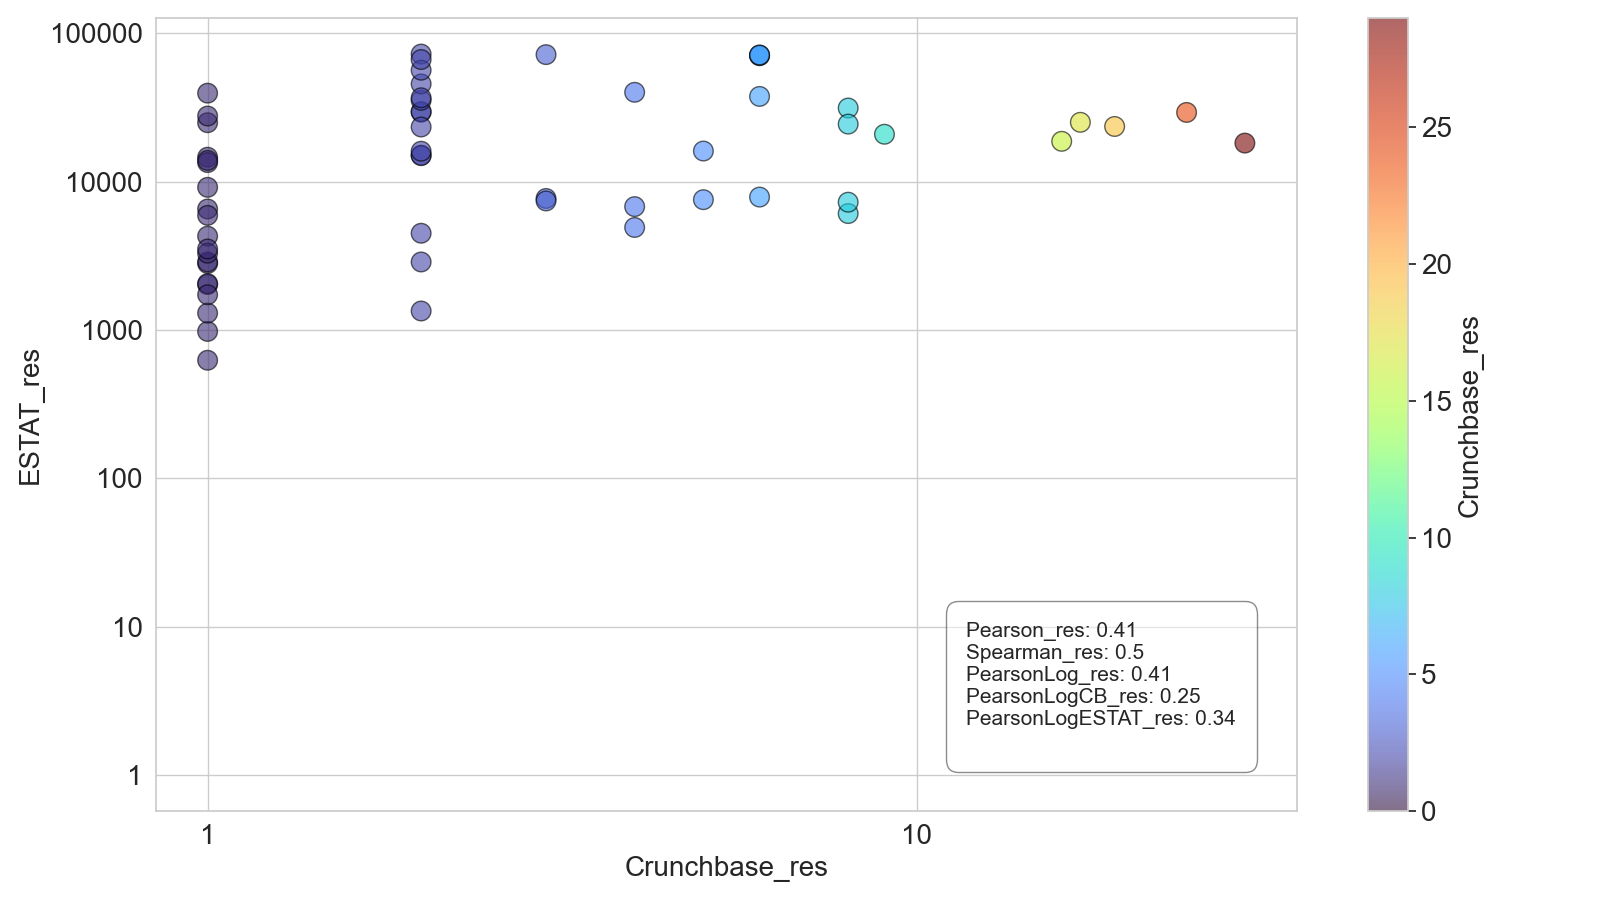
\includegraphics[width=1.0\textwidth]{images/flows/aggregated/filtered_nationality/ita/ESTAT_res_True.png}
        \caption{Flussi residenti}
        \label{fig:italia_res_true}
    \end{subfigure}
    \caption{Confronto dei flussi di emigranti, dall'Italia, di Crunchbase con Eurostat (gli altri stati sono aggregati per zone, periodo 2010 al 2020).}
    \label{fig:italiatrue}
\end{figure}
Nella Figura \ref{fig:italia_nat_true} viene mostrato il confronto dei flussi di emigranti di nazionalità Italiana tra Crunchbase ed Eurostat. Gli stati oltre all'Italia vengono aggregati per zona geografica. Si nota una correlazione di Pearson di 0.55, l'indice di Spearman indica un valore di 0.56. Ponendo i soli dati Eurostat in scala logaritmica la correlazione di Pearson ottiene un valore di 0.58.

La Figura \ref{fig:italia_res_true} mostra i flussi migratori dei residenti in Italia. La correlazione di Pearson è di 0.4, invece l'indice di Spearman è di 0.5. Interventi di trasformazione in scala logaritmica di uno dei due insiemi (Eurostat e Crunchbase) portano a correlazioni di Pearson uguali o inferiori (0.41, 0.25, 0.34).

Entrambi i casi di confronto indicano una correlazione discreta tra i flussi di Crunchbase ed Eurostat per gli utenti emigrati dall'Italia. Si nota dalla barra laterale come il valore massimo di emigranti altamente qualificati dall'Italia nei flussi Crunchbase è intorno alle 25 unità. 

\paragraph{Flussi d'immigrazione in Italia}
\label{toIta_flows}
\begin{figure}[tb]
    \centering
    \begin{subfigure}{\textwidth}
        \centering
        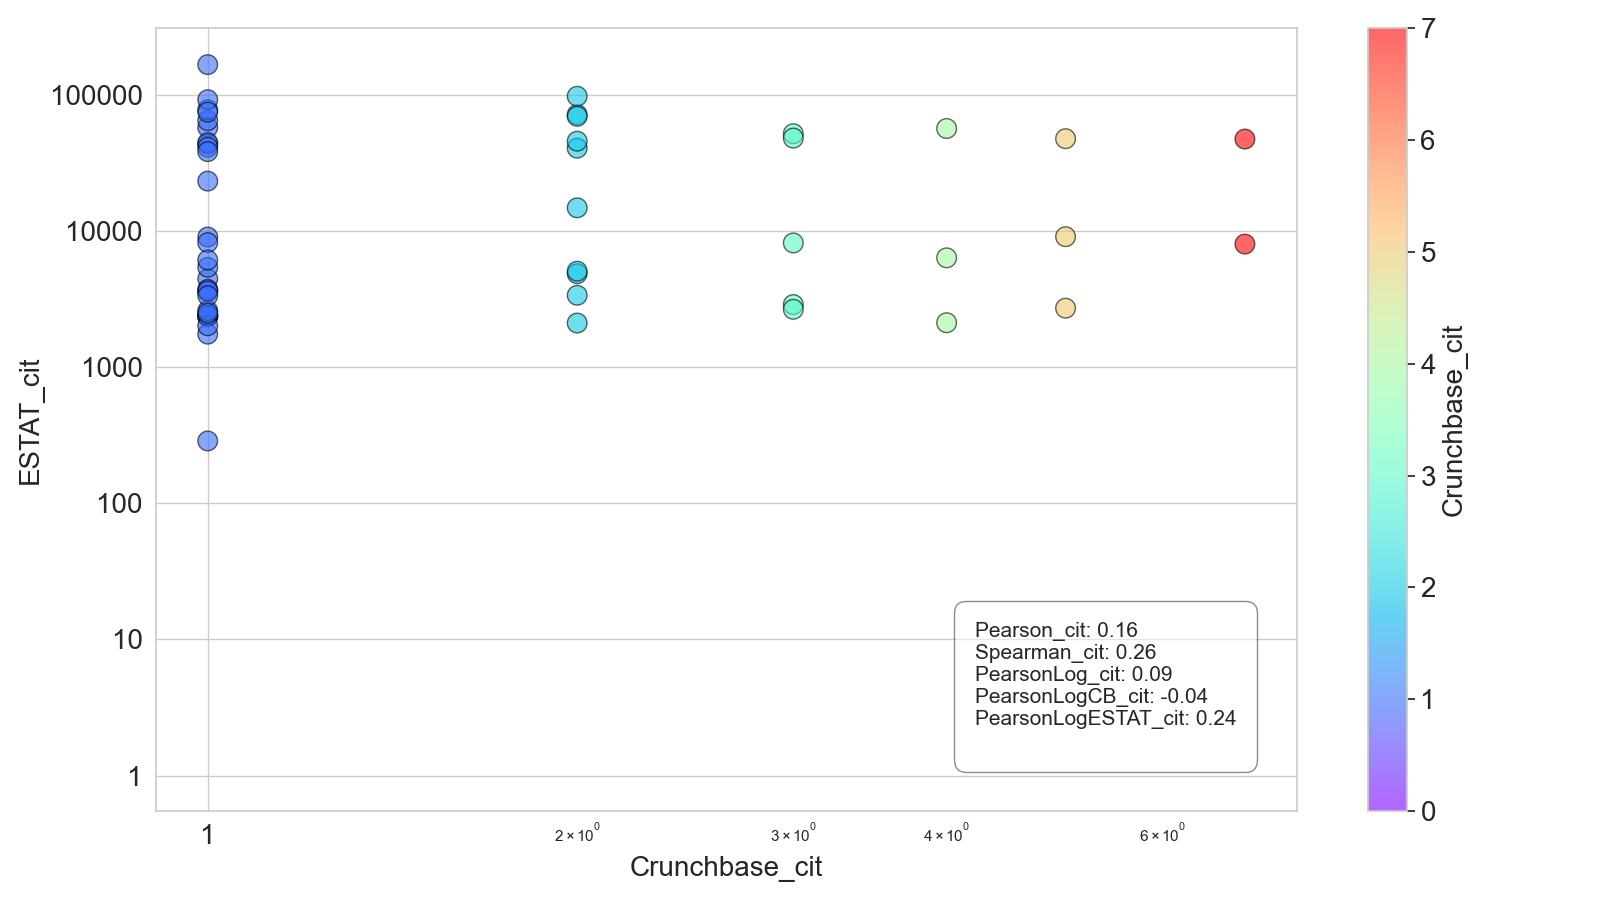
\includegraphics[width=1.0\textwidth]{images/flows/aggregated/filtered_destination/ita/ESTAT_cit_True.png}
        \caption{Flussi cittadini}
        \label{fig:italia_dest_true_cit}
    \end{subfigure}
    \begin{subfigure}{\textwidth}
        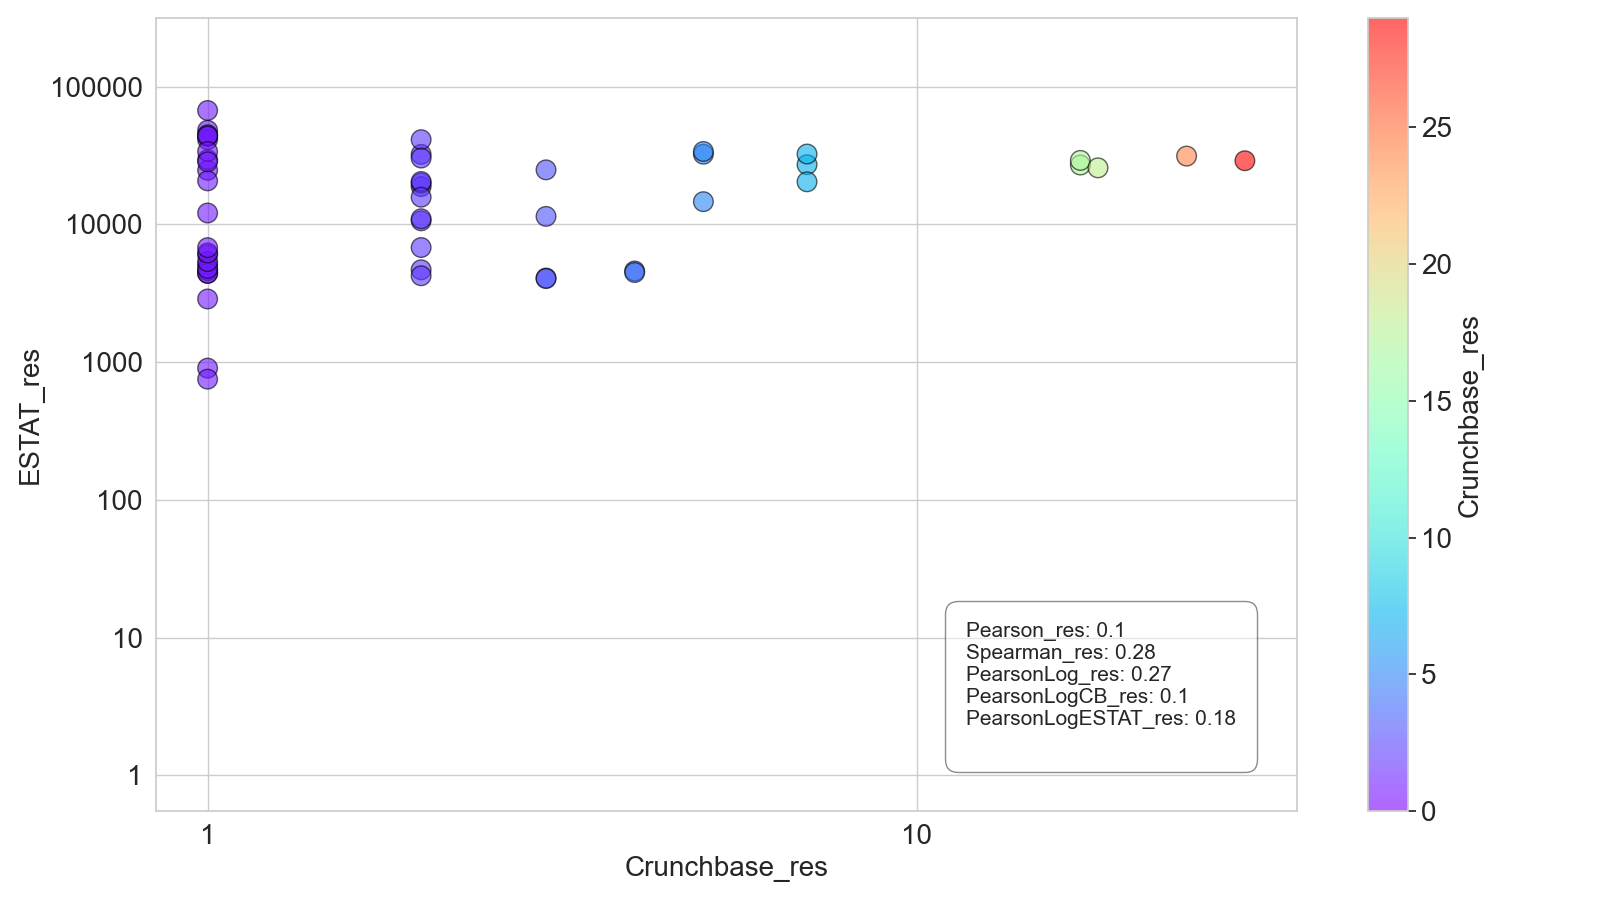
\includegraphics[width=1.0\textwidth]{images/flows/aggregated/filtered_destination/ita/ESTAT_res_True.png}
        \caption{Flussi residenti}
        \label{fig:italia_dest_true_res}
    \end{subfigure}
    \caption{Confronto dei flussi di immigranti in Italia, tra Crunchbase ed Eurostat (gli altri stati sono aggregati per zone, periodo 2010 al 2020).}
\end{figure}
Nella Figura \ref{fig:italia_dest_true_cit} viene mostrato il flusso di cittadini esteri che hanno migrato in Italia. 
La correlazione di Pearson è di 0.16, l'indice di Spearman è di 0.26. Ponendo in scala logaritmica i flussi dei cittadini in Eurostat la correlazione di Pearson incrementa fino a 0.24. Il valore massimo di flussi di cittadini esteri immigrati in Italia incontrato in Crunchbase è di 7 persone. 
In Figura \ref{fig:italia_dest_true_res} è presente il grafico dei flussi dei residenti all'estero che hanno migrato in Italia. Il valore della correlazione di Pearson è di 0.01, ed incrementa fino a 0.18 se poniamo i flussi di Eurostat in scala logaritmica. L'indice di Spearman ha invece un valore di 0.18. Il valore massimo di residenti all'estero immigrati in Italia in Crunchbase è di poco più di 25 persone. Inoltre, i valori dei coefficienti di Pearson e di Spearman per cittadini e residenti indicano che non vi è correlazione tra i dati Crunchbase ed i dati Eurostat per questo caso di studio.

\FloatBarrier

\subsection{Caso di studio: Gran Bretagna}
\label{CASOFLUSSIGBR}
In questa sezione si analizzano in particolare i flussi di migranti da e verso la Gran Bretagna su tutto il periodo dei dati collezionati (dal 2010 al 2020). Il confronto viene fato con i dati ottenuti da UN unito ad Eurostat.
\paragraph{Flussi di emigranti dalla Gran Bretagna}
\label{gbr_flows}
\begin{figure}[!ht]
    \centering
    \begin{subfigure}{\textwidth}
        \centering
        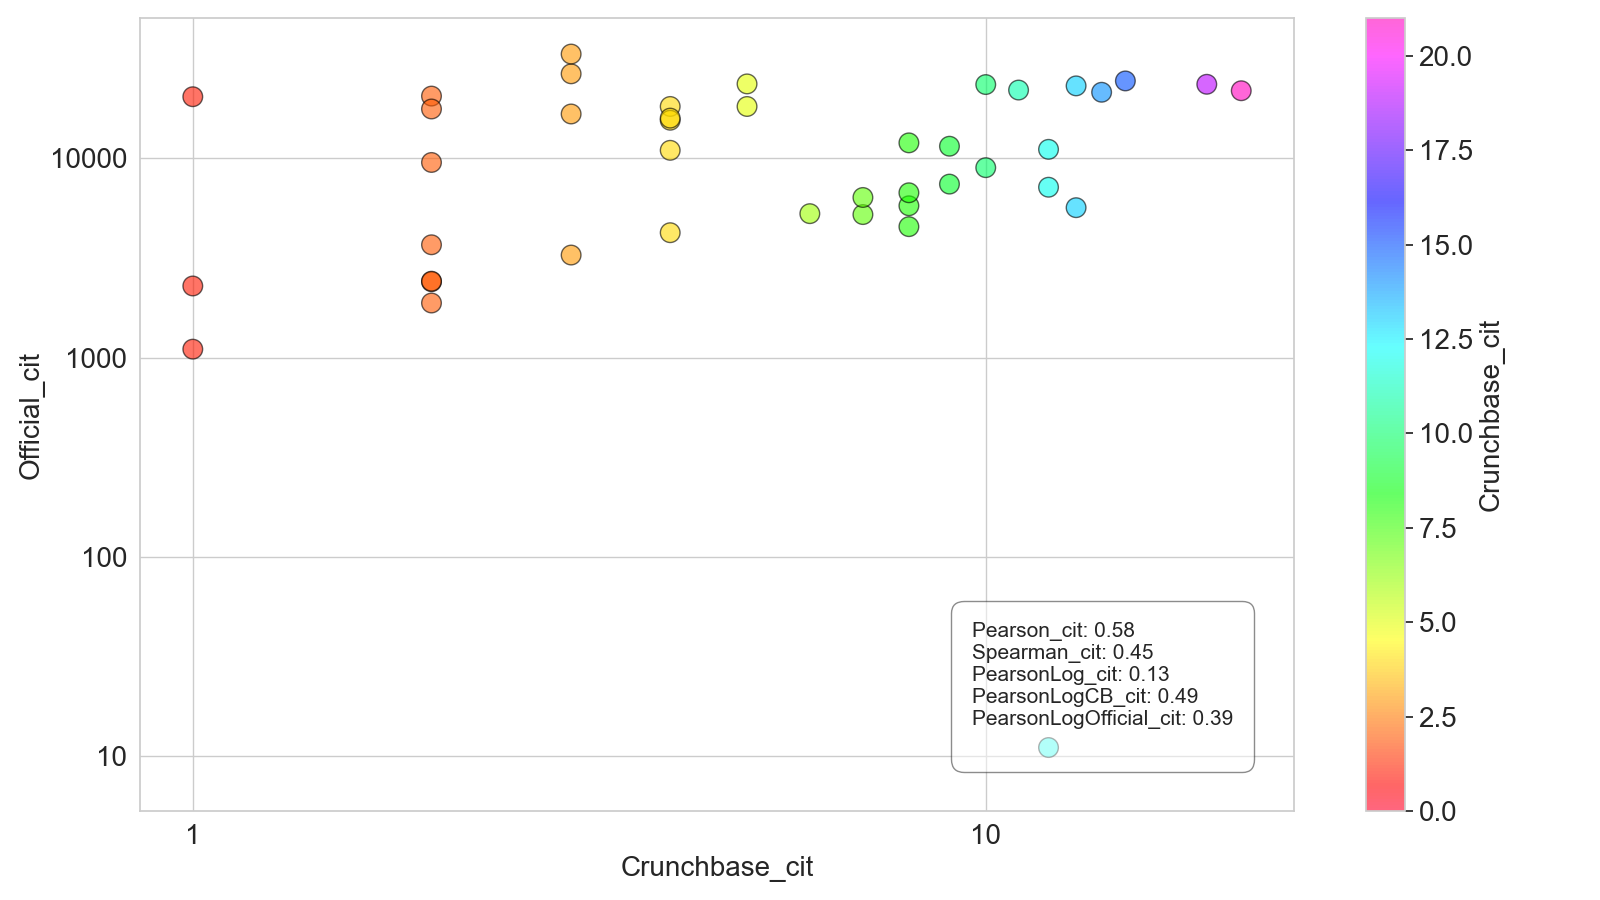
\includegraphics[width=0.95\textwidth]{images/flows/aggregated/filtered_nationality/gbr/Official_cit_True.png}
        \caption{Flussi cittadini}
        \label{fig:gbr_nat_true}
    \end{subfigure}
    \begin{subfigure}{\textwidth}
        \centering
        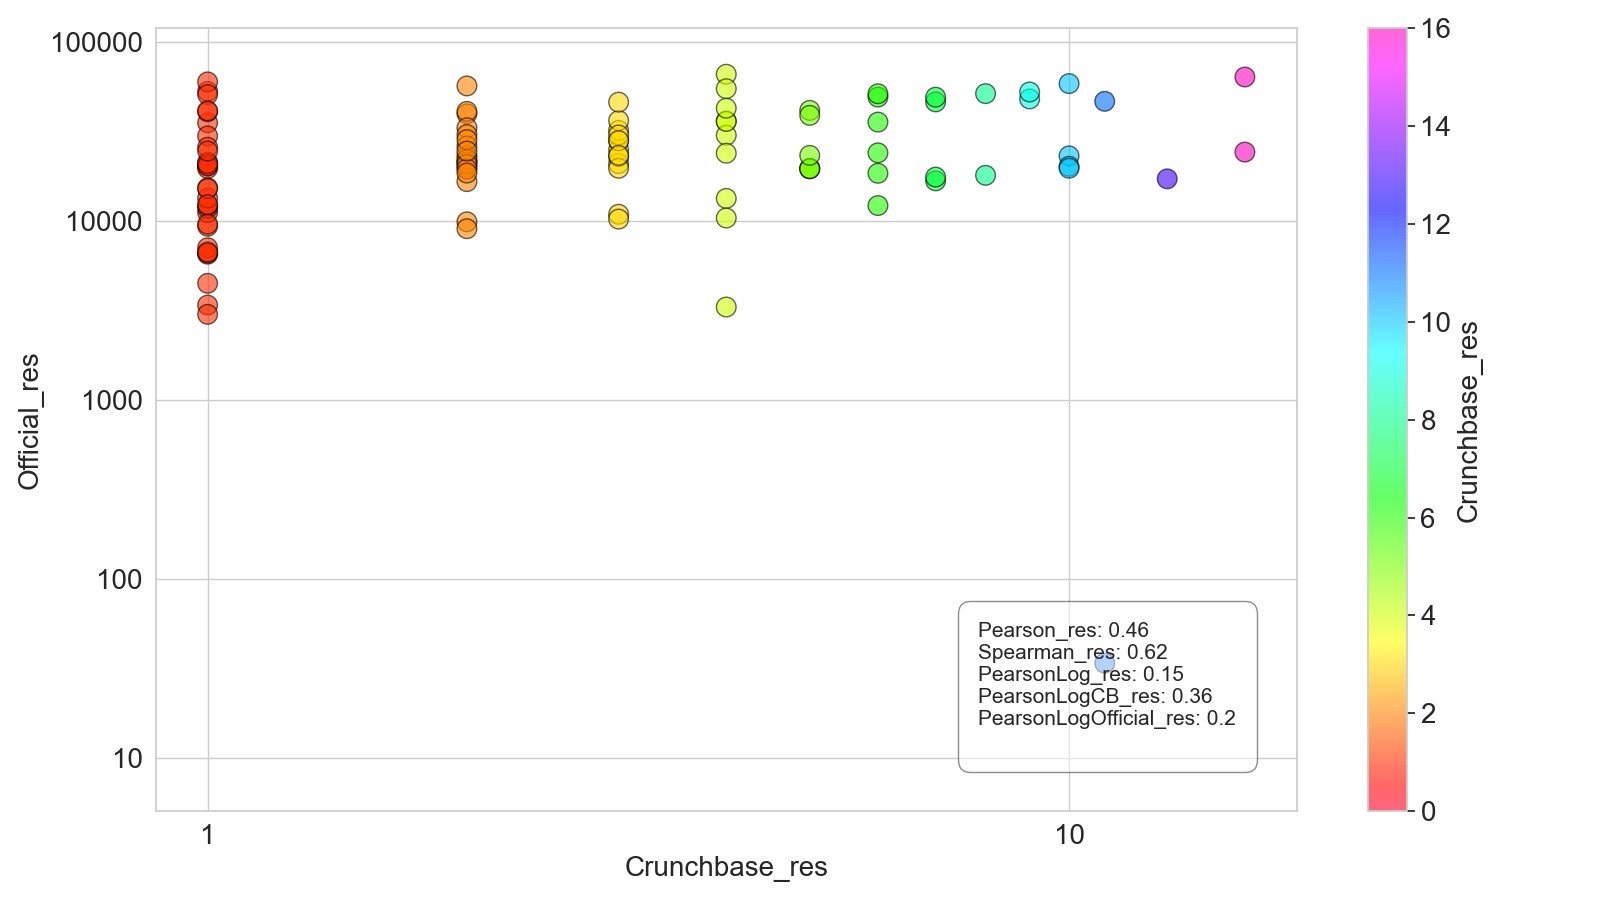
\includegraphics[width=0.95\textwidth]{images/flows/aggregated/filtered_nationality/gbr/Official_res_True.png}
        \caption{Flussi residenti}
        \label{fig:gbr_res_true}
    \end{subfigure}
    \caption{Confronto dei flussi di emigranti britannici, tra Crunchbase e UN unito Eurostat (gli altri stati sono aggregati per zone geografiche, il periodo è 2010-2020).}
    \label{fig:gbr_True}
\end{figure}
In Figura \ref{fig:gbr_nat_true} viene mostrato il confronto tra i flussi dei cittadini britannici che emigrano, tra  Crunchbase e UN unito Eurostat. 
La correlazione di Pearson ottenuta è di 0.58, invece l'indice di Spearman ha un valore di 0.45. Ponendo gli insiemi in scale logaritmiche la correlazione di Pearson decrementa il suo valore in tutti i casi (0.13, 0.49, 0.39). 
Il grafico in Figura \ref{fig:gbr_res_true} mostra i flussi dei residenti in Gran Bretagna, che hanno emigrato. La correlazione di Pearson ha un valore di 0.46 come per il grafico dei cittadini in Figura \ref{fig:gbr_nat_true}. L'indice di Spearman ha invece un valore di 0.62. Inoltre, utilizzare scale logaritmiche sui flussi (Ufficiali o di Crunchbase) porta a valori inferiori alla correlazione normale. Entrambi i coefficienti indicano una correlazione discreta tra i dati Crunchbase e UN unito Eurostat sia per nativi che residenti della Gran Bretagna che hanno emigrato.
\paragraph{Flussi d'immigrazione in Gran Bretagna}
\label{togbr_flows}
\begin{figure}[tb]
    \centering
    \begin{subfigure}{\textwidth}
        \centering
        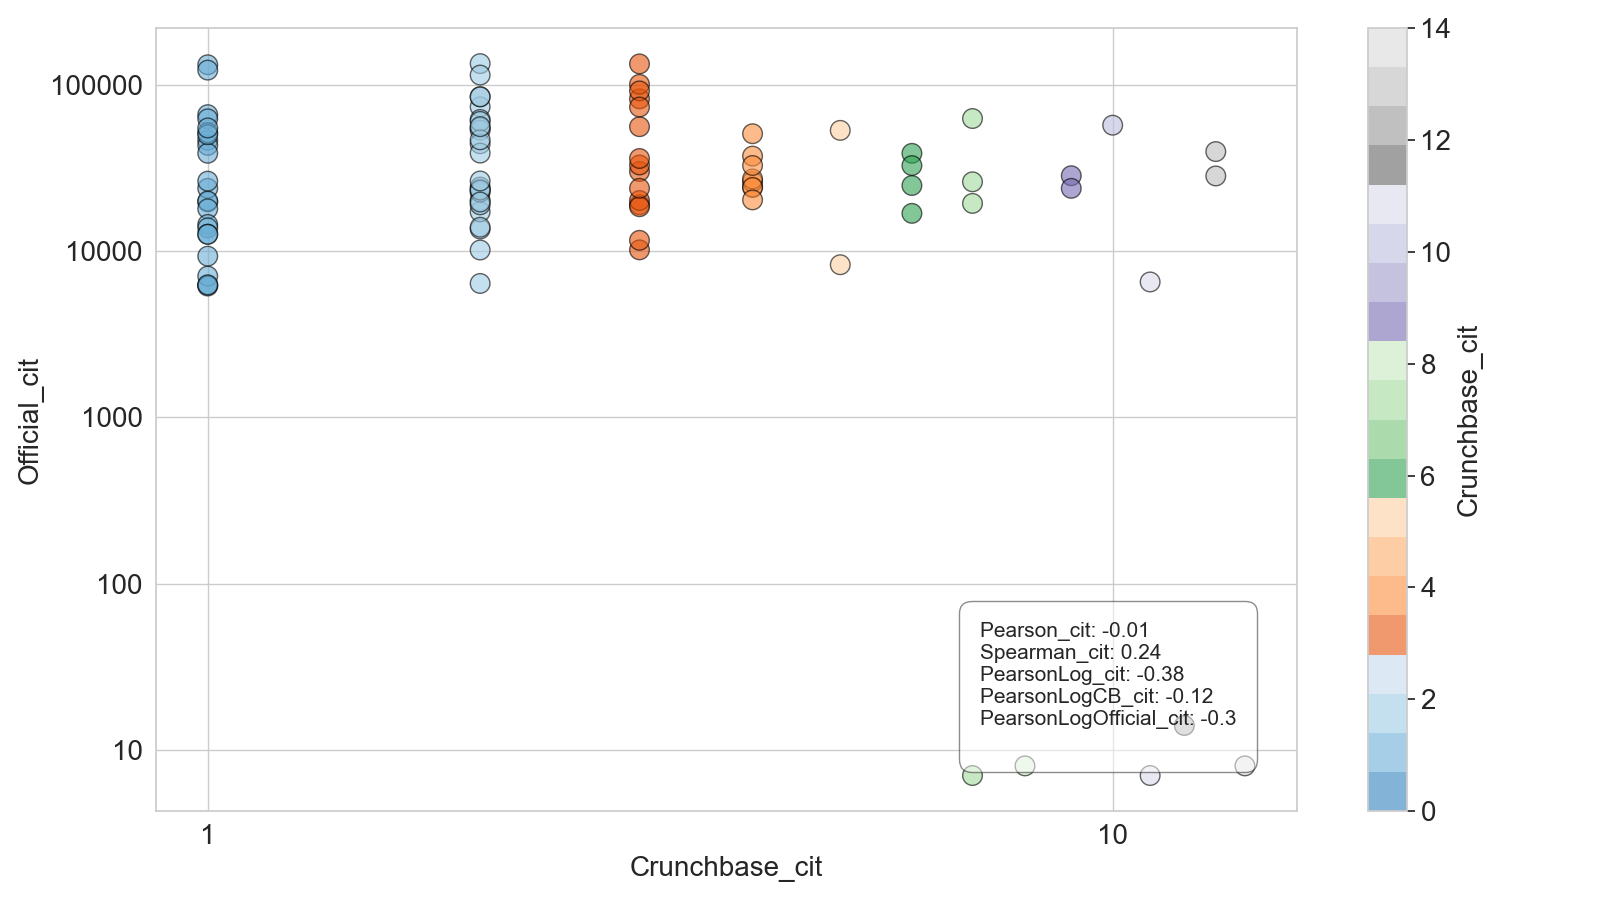
\includegraphics[width=0.9\textwidth]{images/flows/aggregated/filtered_destination/gbr/Official_cit_True.png}
        \caption{Flussi cittadini}
        \label{fig:gbr_dest_true_cit}
    \end{subfigure}
    \begin{subfigure}{\textwidth}
        \centering
        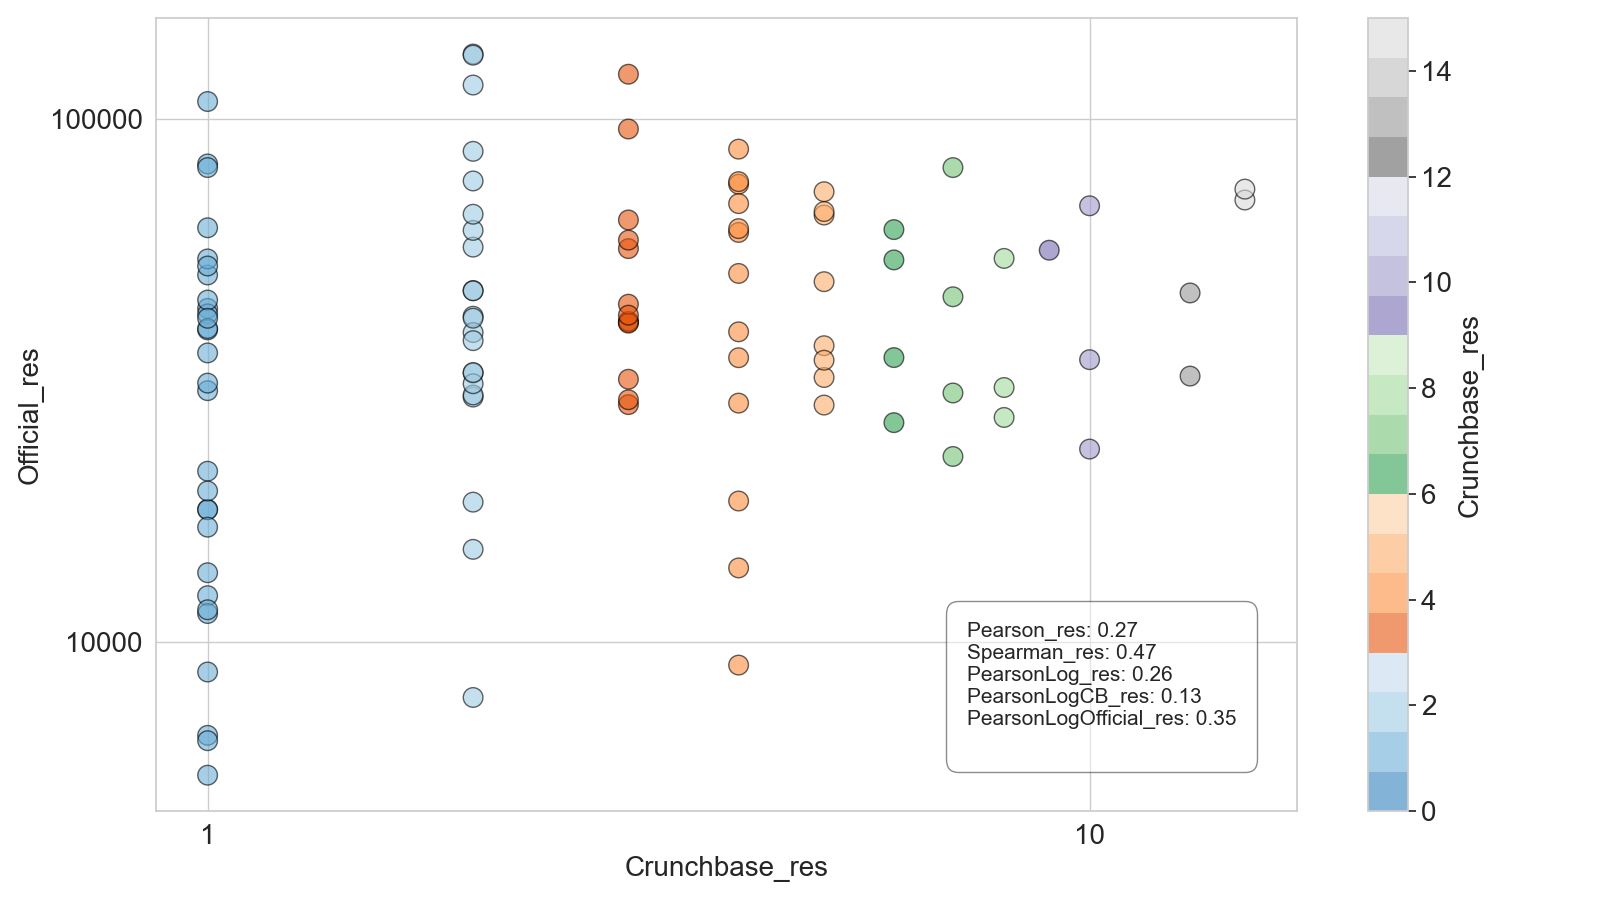
\includegraphics[width=0.9\textwidth]{images/flows/aggregated/filtered_destination/gbr/Official_res_True.png}
        \caption{Flussi residenti}
        \label{fig:gbr_dest_true_res}
    \end{subfigure}
    \caption{Confronto dei flussi di immigranti in Gran Bretagna, tra Crunchbase e UN unito Eurostat (gli altri stati sono aggregati per zone geografiche, il periodo è 2010-2020).}
    \label{fig:gbr_dest_true}
\end{figure}
Nel grafico in Figura \ref{fig:gbr_dest_true_cit} vengono confrontati i flussi di cittadini esteri che migrano in Gran Bretagna, tra Crunchbase e UN unito Eurostat. La correlazione di Pearson è di 0.1, invece l'indice di Spearman ha valore 0.24. Ponendo in scala logaritmica entrambe le fonti dei flussi (UN unito Eurostat e Crunchbase) si ha una correlazione di Pearson negativa di -0.12. Questi valori indicano che non sia presente correlazione tra i dati Crunchbase ed i dati di UN unito Eurostat, per i flussi di cittadini esteri immigrati in Gran Bretagna.
La Figura \ref{fig:gbr_dest_true_res} mostra i flussi degli immigranti in Gran Bretagna. La correlazione di Pearson è di 0.27 l'indice di Spearman è di 0.47. Utilizzando una scala logaritmica per i flussi dei dati ufficiali (UN unito ad Eurostat) si ha una correlazione di Pearson di 0.35.
La correlazione di Spearman indica che ci sia una correlazione positiva discreta tra i dati confrontati.
\FloatBarrier

\subsection{Discussione}
I flussi dei dati collezionati attraverso Crunchbase sono significativi per l'Europa ed il Nord America come visto nella sezione \ref{flowscrunch}. 
La correlazione con i flussi in Eurostat è debole, in alcuni casi anche discreta (Sezione \ref{ESTAT_aggregated}) se aggregati, i flussi in Eurostat però non presentano dati per la Gran Bretagna \cite{MIMIDOC}. 
La correlazione dei flussi con UN non è presente, come abbiamo visto nell'analisi (Sezioni \ref{UN_original}, \ref{UN_aggregated}). 
L'unione dei flussi UN con i flussi Eurostat non ha correlazione per Pearson nell'analisi effettuata, ma per l'indice di Spearman questa è presente in forma debole (Sezione \ref{UNunionEstatflows}). 
Tra i casi di studio affrontati l'emigrazione di cittadini e residenti Italiani presenta una correlazione discreta (Sezione \ref{ita_flows}), con un numero massimo di migranti pari a 20. 
L'immigrazione verso l'Italia non presenta correlazione con i dati Eurostat (Sezione \ref{toIta_flows}). 
Per la Gran Bretagna i flussi presentano una correlazione discreta per gli emigranti (Sezione \ref{gbr_flows}). I flussi di immigranti in Gran Bretagna invece non presentano correlazione per i cittadini di altre nazioni. Per i residenti di altre nazioni che si spostano in Gran Bretagna la correlazione è discreta (Sezione \ref{togbr_flows}). 